\subsection{Simulation of \vg\ Processes}
\label{sec:vgmc}

The \zinvg\ and \wlng\ background contributions are modeled using MC simulations.
Samples generated at the leading order (LO) in QCD by \MADGRAPH5 with up to two additional partons and a generator-level requirement of $\ETg > 130\GeV$ are employed for this purpose.

A study using an aMC@NLO sample with high \ETg\ threshold confirms that the predicted kinematic distributions would not change drastically by using the NLO sample. 
Figures~\ref{fig:zg_nlo_lo} and \ref{fig:wg_nlo_lo} show the comparisons of the aMC@NLO samples\footnote{These samples were privately produced.} and the \MADGRAPH5 samples used for the background estimation in the key kinematic distributions.

\begin{figure}[htbp]
  \centering
  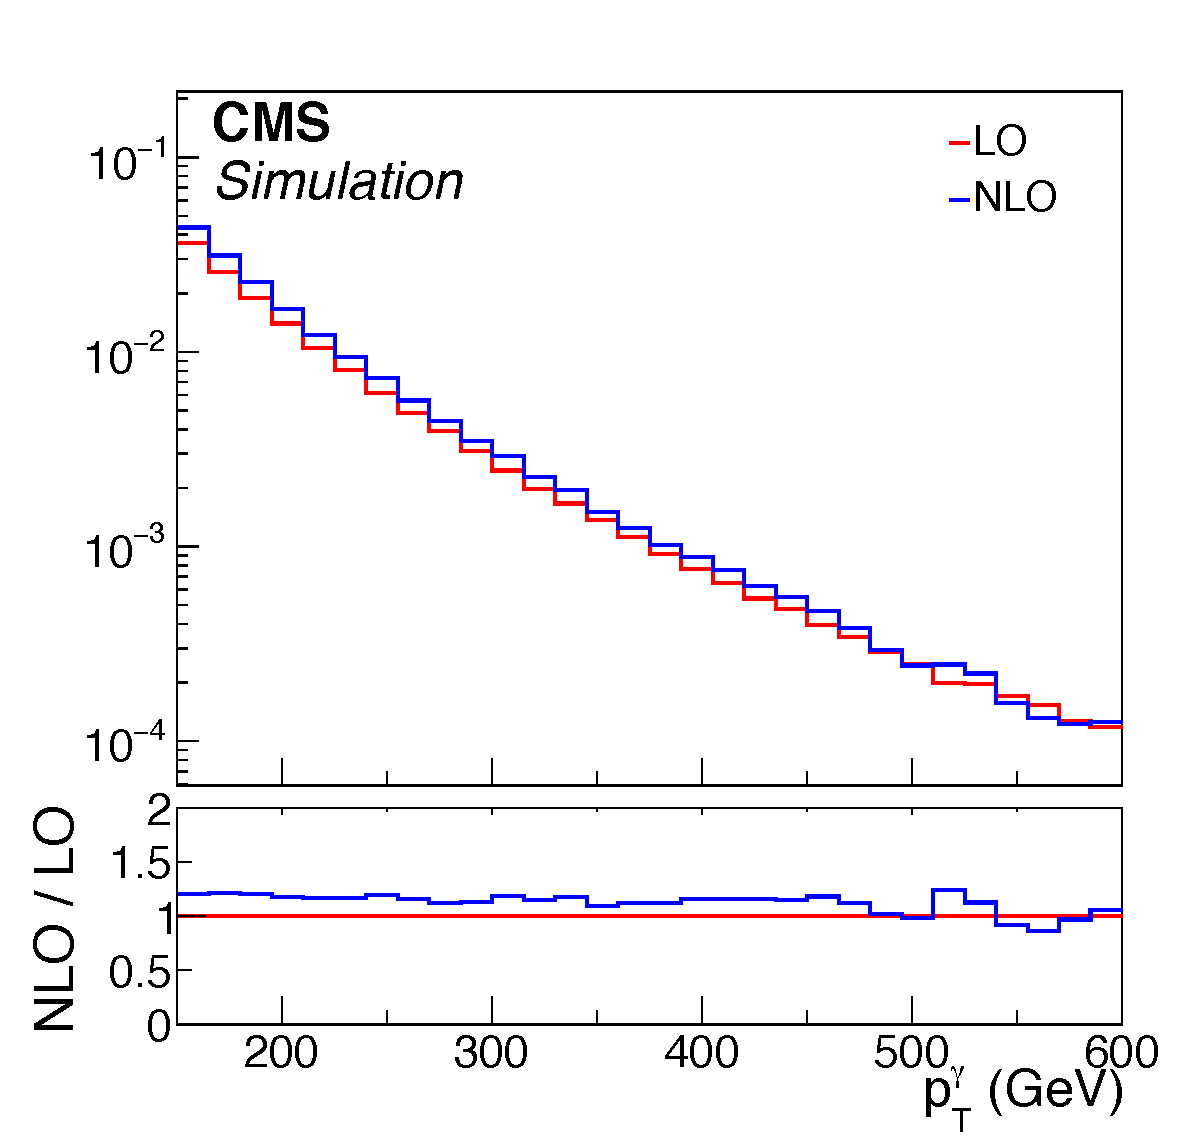
\includegraphics[width=0.32\textwidth]{Analysis/Figures/kfactor/ZG_ptg.pdf}
  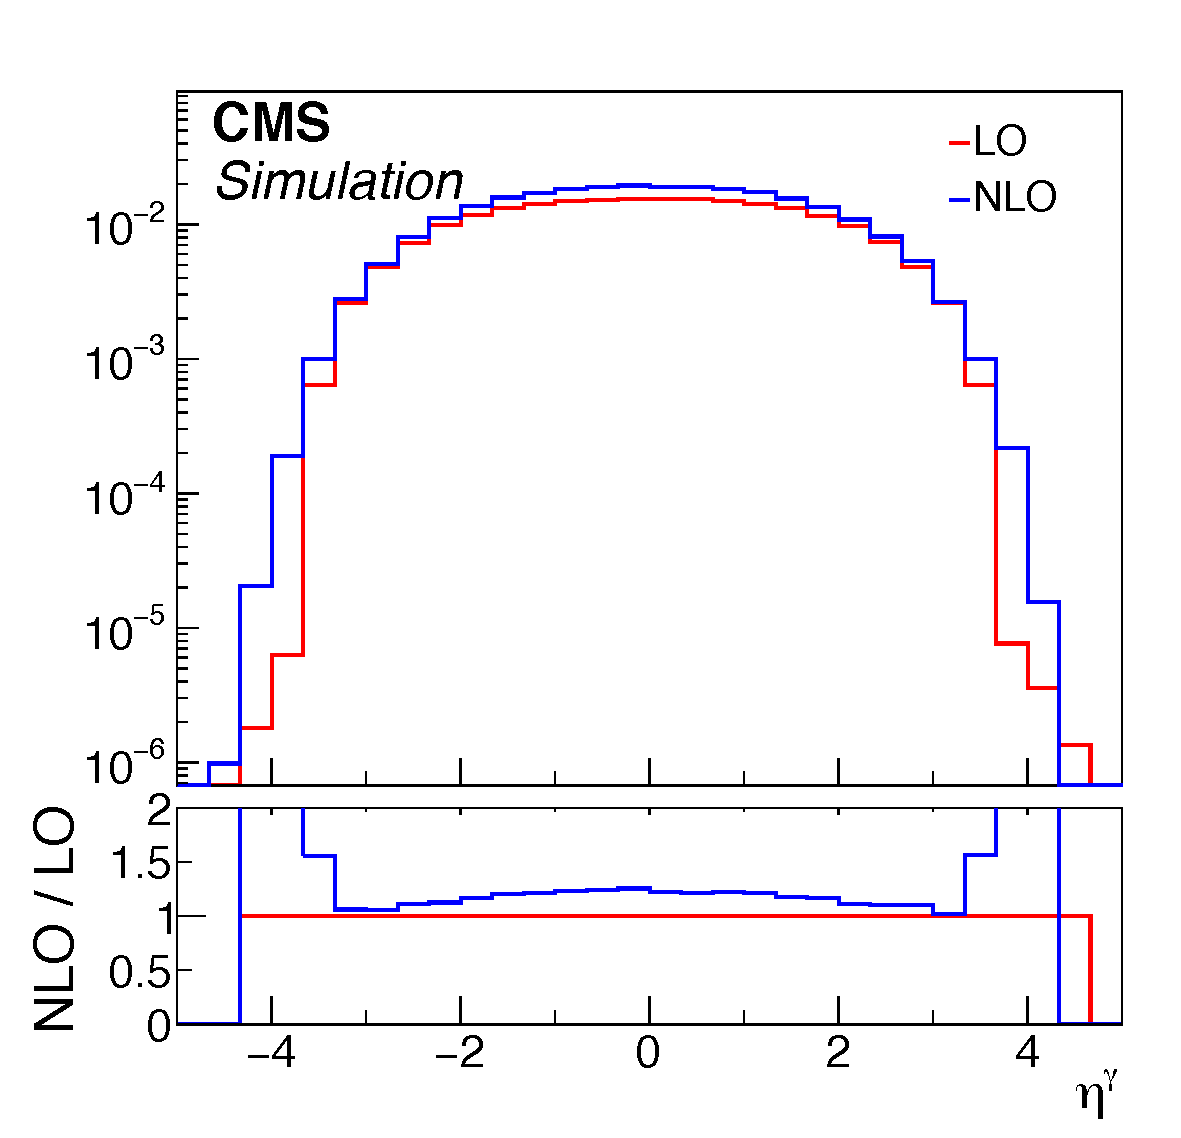
\includegraphics[width=0.32\textwidth]{Analysis/Figures/kfactor/ZG_etag.pdf}
  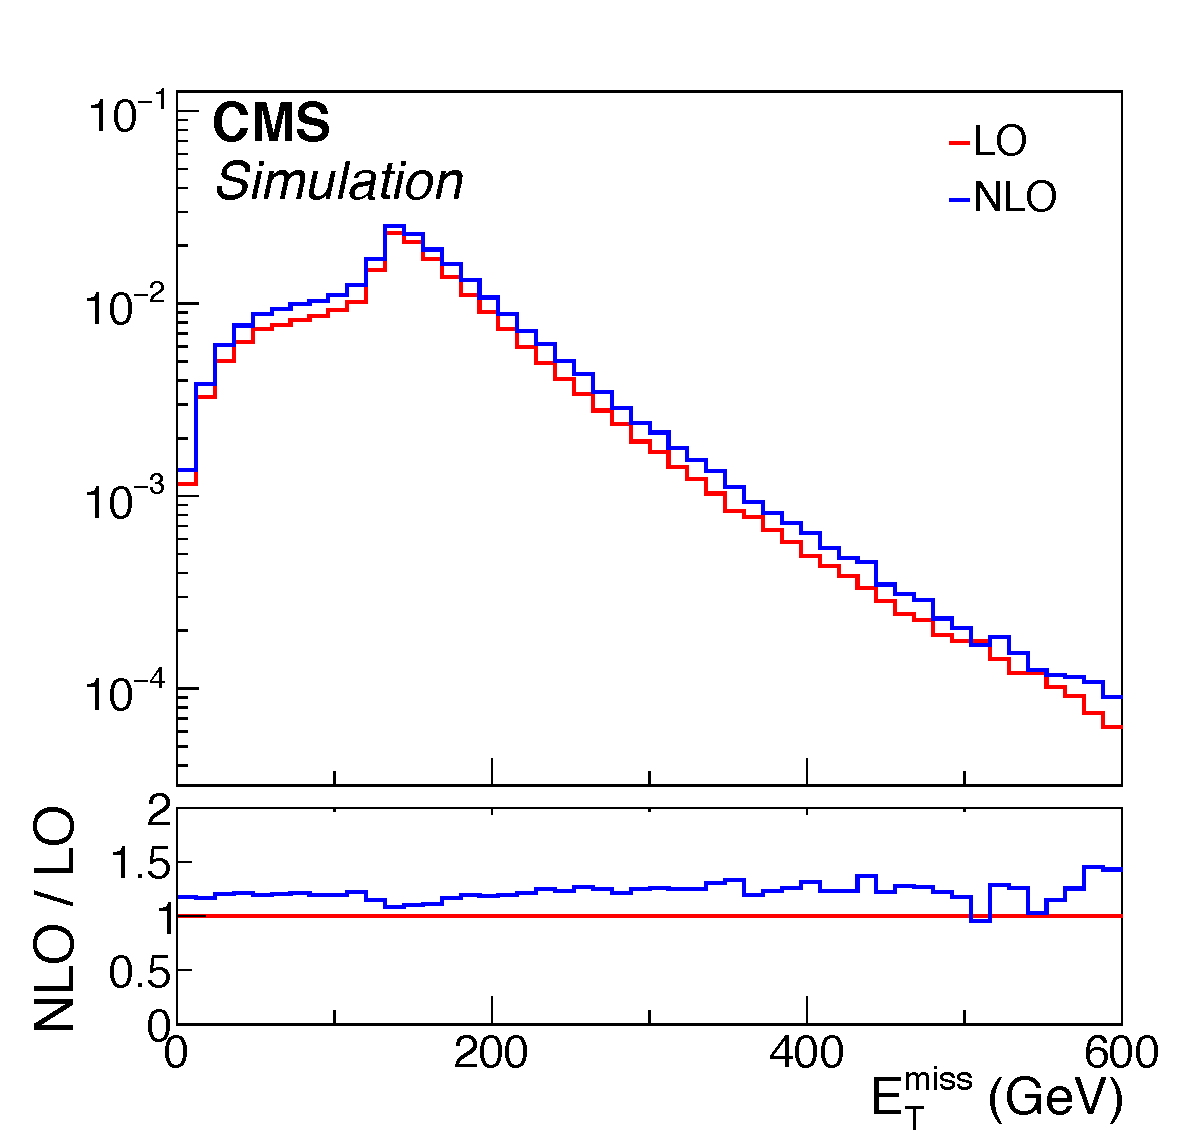
\includegraphics[width=0.32\textwidth]{Analysis/Figures/kfactor/ZG_met.pdf}
  \caption{
    Distributions of \ETg\ (left), $\eta^{\Pgg}$ (middle), and $\pt^{\PZ}$ (right) in \zinvg\ process from the private aMC@NLO sample (blue) and the LO sample used for background prediction (red) along with the NLO / LO ratios.
  }
  \label{fig:zg_nlo_lo}
\end{figure}
\begin{figure}[htbp]
  \centering
  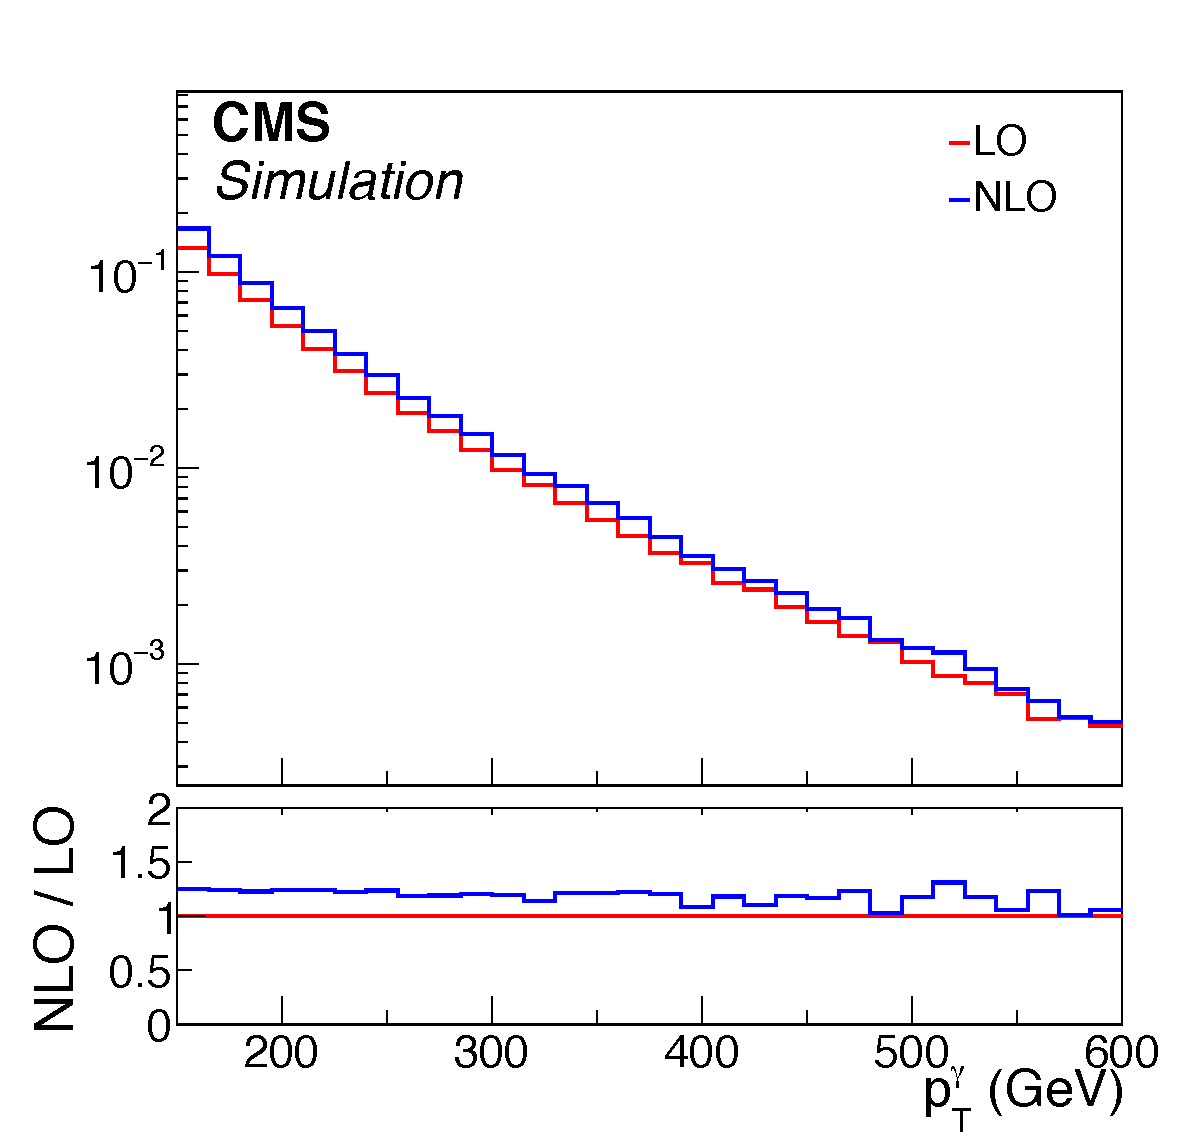
\includegraphics[width=0.32\textwidth]{Analysis/Figures/kfactor/WG_ptg.pdf}
  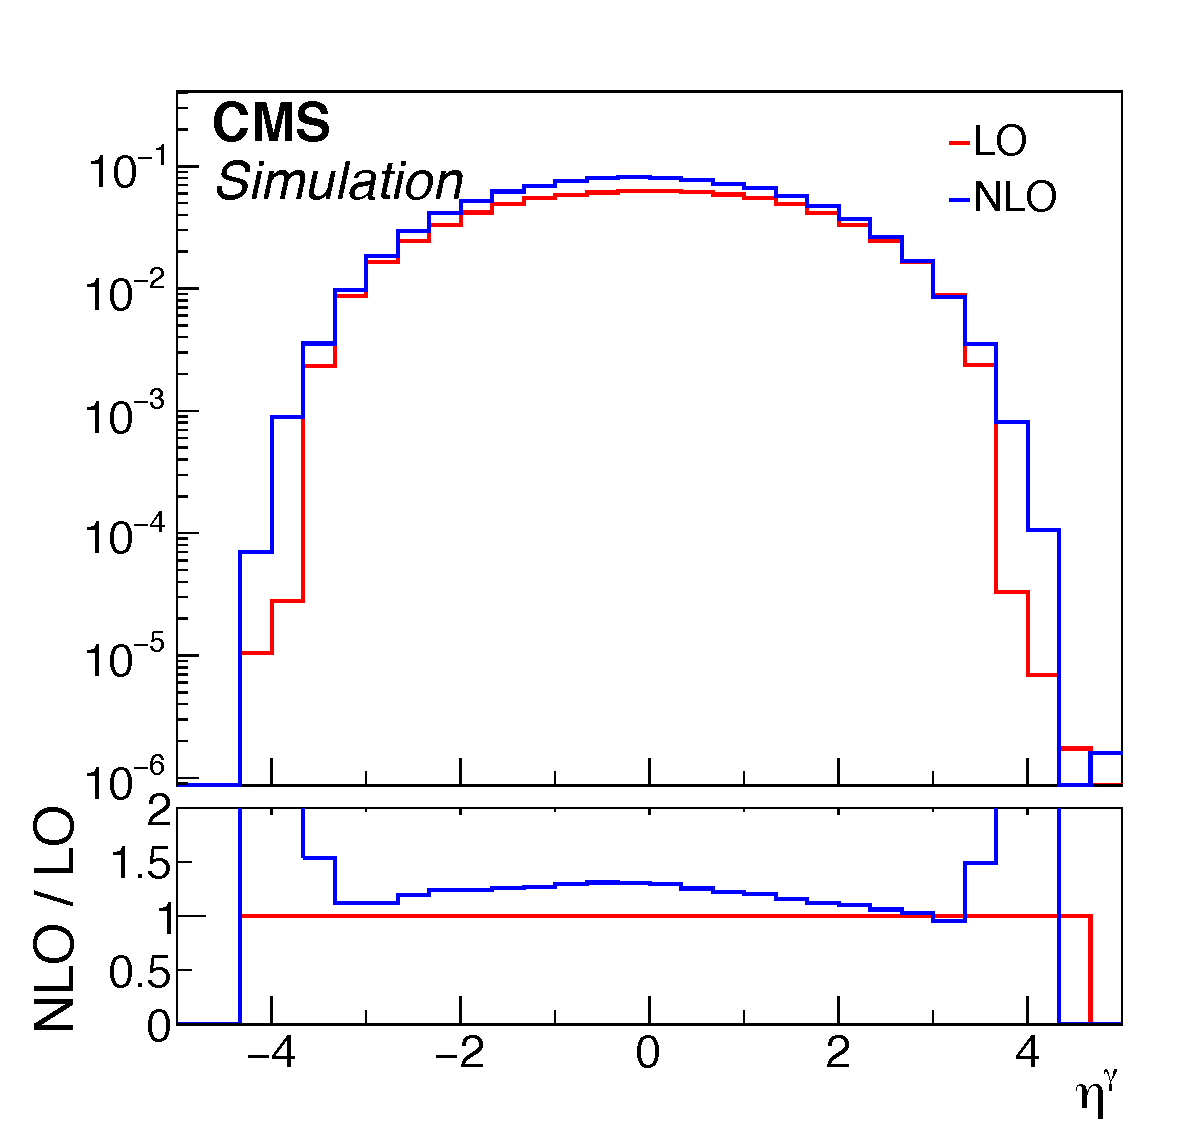
\includegraphics[width=0.32\textwidth]{Analysis/Figures/kfactor/WG_etag.pdf}
  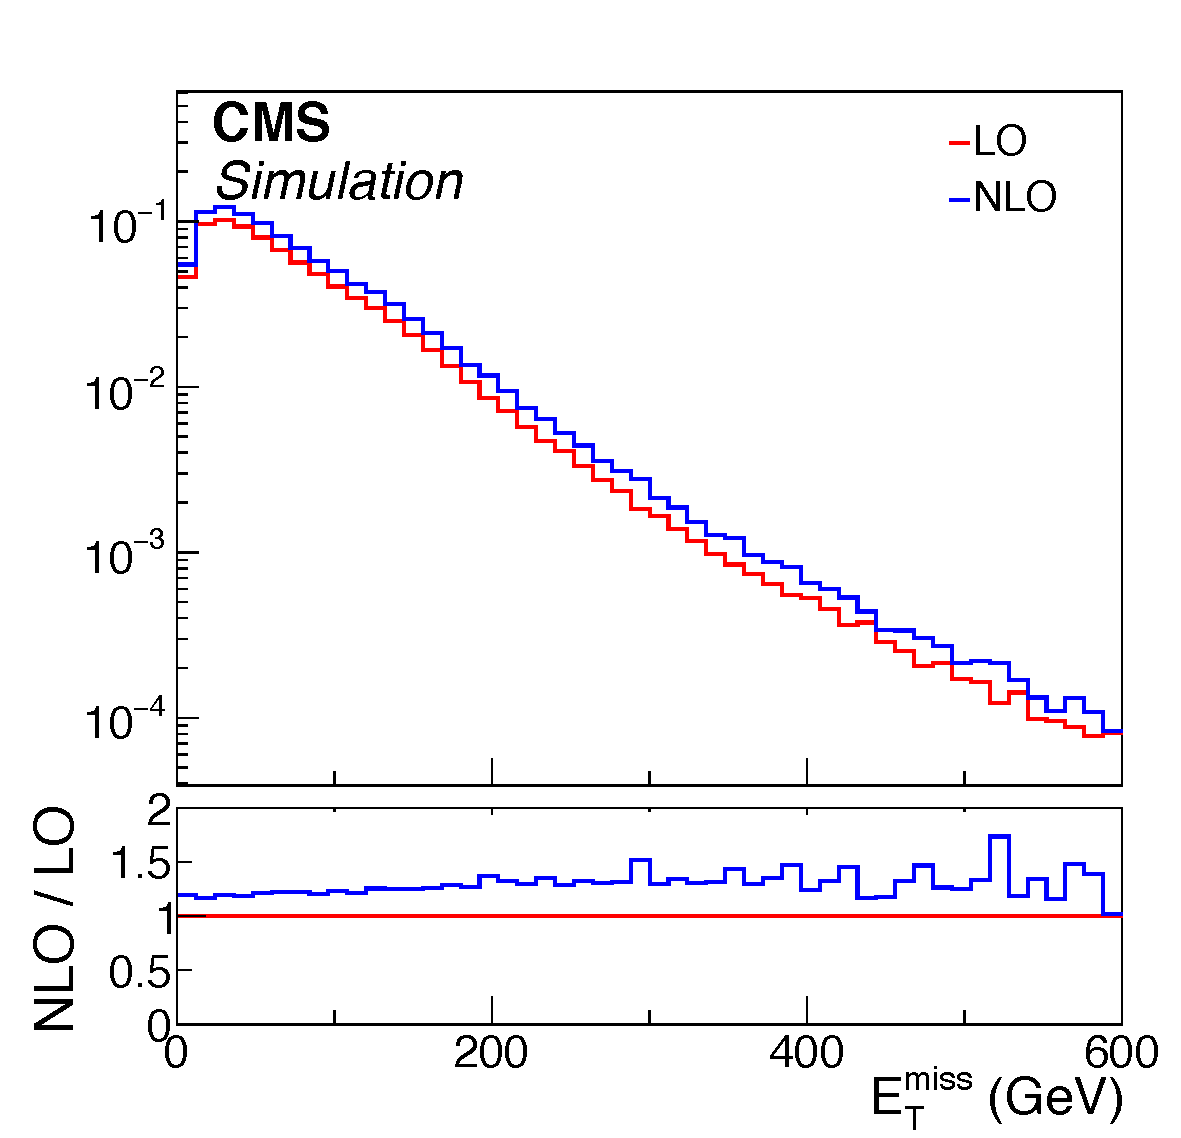
\includegraphics[width=0.32\textwidth]{Analysis/Figures/kfactor/WG_met.pdf}
  \caption{
    Distributions of \ETg\ (top left), $\eta^{\Pgg}$ (top right), and $\pt^{\PW}$ (bottom left) in \wlng\ process from the private aMC@NLO sample (blue) and the LO sample used for background prediction (red) along with the NLO / LO ratios.
  }
  \label{fig:wg_nlo_lo}
\end{figure}

To approximate the QCD higher-order effects, \zinvg\ and \wlng\ events are reweighted with \ETg\ by the factors given in Tab.~\ref{tab:zg_kfactors}. 
These factors are the ratios of QCD next-to-next-to leading order (NNLO) differential cross sections calculated by Grazzini et al.~\cite{Bozzi:2010xn} to the LO cross sections given in the centrally produced samples. 
Note that the denominator cross section includes contributions from processes with up to two additional partons, and is therefore not a LO cross section in the strict sense of the word. V\Pgg\ k-factors found in literature are $\gg 1$ at high \ETg, if the denominator only accounts for the cross section of $\Pq\Paq\rightarrow\mathrm{V}\Pgg$ process.

\begin{table}
  \begin{center}
    \begin{tabular}{ l | r | r }
      \ETg range (GeV) & \zinvg & \wlng \\
      \hline
      $[175, 190]$ & 1.44 & 1.40 \\
      $[190, 250]$ & 1.41 & 1.37 \\
      $[250, 400]$ & 1.35 & 1.31 \\
      $[400, 700]$ & 1.29 & 1.26 \\
      $[700, \infty)$ & 1.15 & 1.15 \\
    \end{tabular}
    \caption{Correction factors \kqcd\ for \zinvg\ and \wlng\ samples.}
    \label{tab:zg_kfactors}
  \end{center}
\end{table}

Higher-order electroweak correction factors are also applied as a function of \ETg. 
Out of various electroweak higher-order effects, ones that can give sizeable
($\gg\mathcal{O}(\alpha)$) corrections to the cross section are the Sudakov suppression at high boson \pt\ and potentially the addition of photon-induced scattering processes~\cite{Denner:2014bna,Denner:2015fca}. 
We apply the correction factors shown in Figure~\ref{fig:ewk_correction}, which are the combinations of Sudakov suppression factors and photon-induced enhancements, and are provided by the authors of Ref.~\cite{Denner:2015fca} in addition to the NNLO QCD correction.

\begin{figure}[htbp]
  \centering
  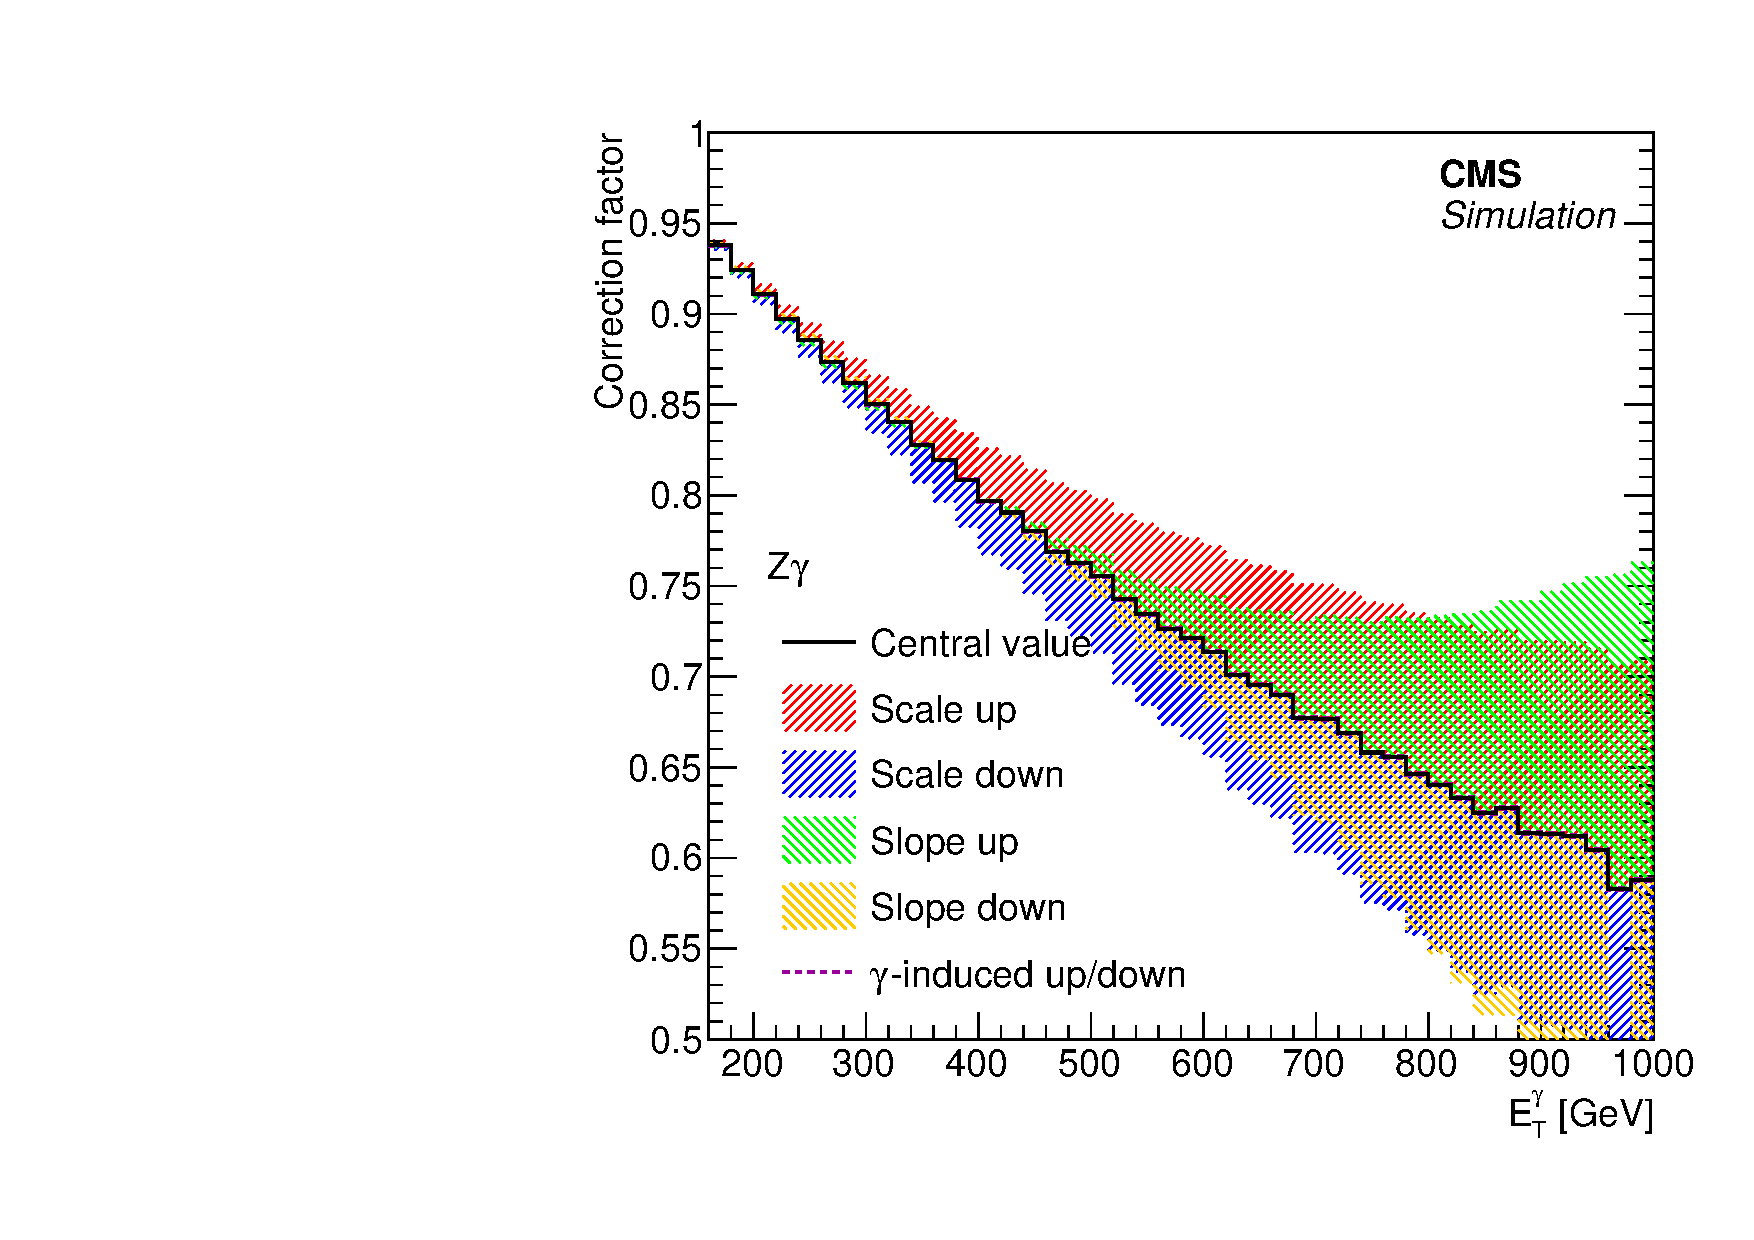
\includegraphics[width=0.32\textwidth]{Analysis/Figures/ewkcorr/zg.pdf}
  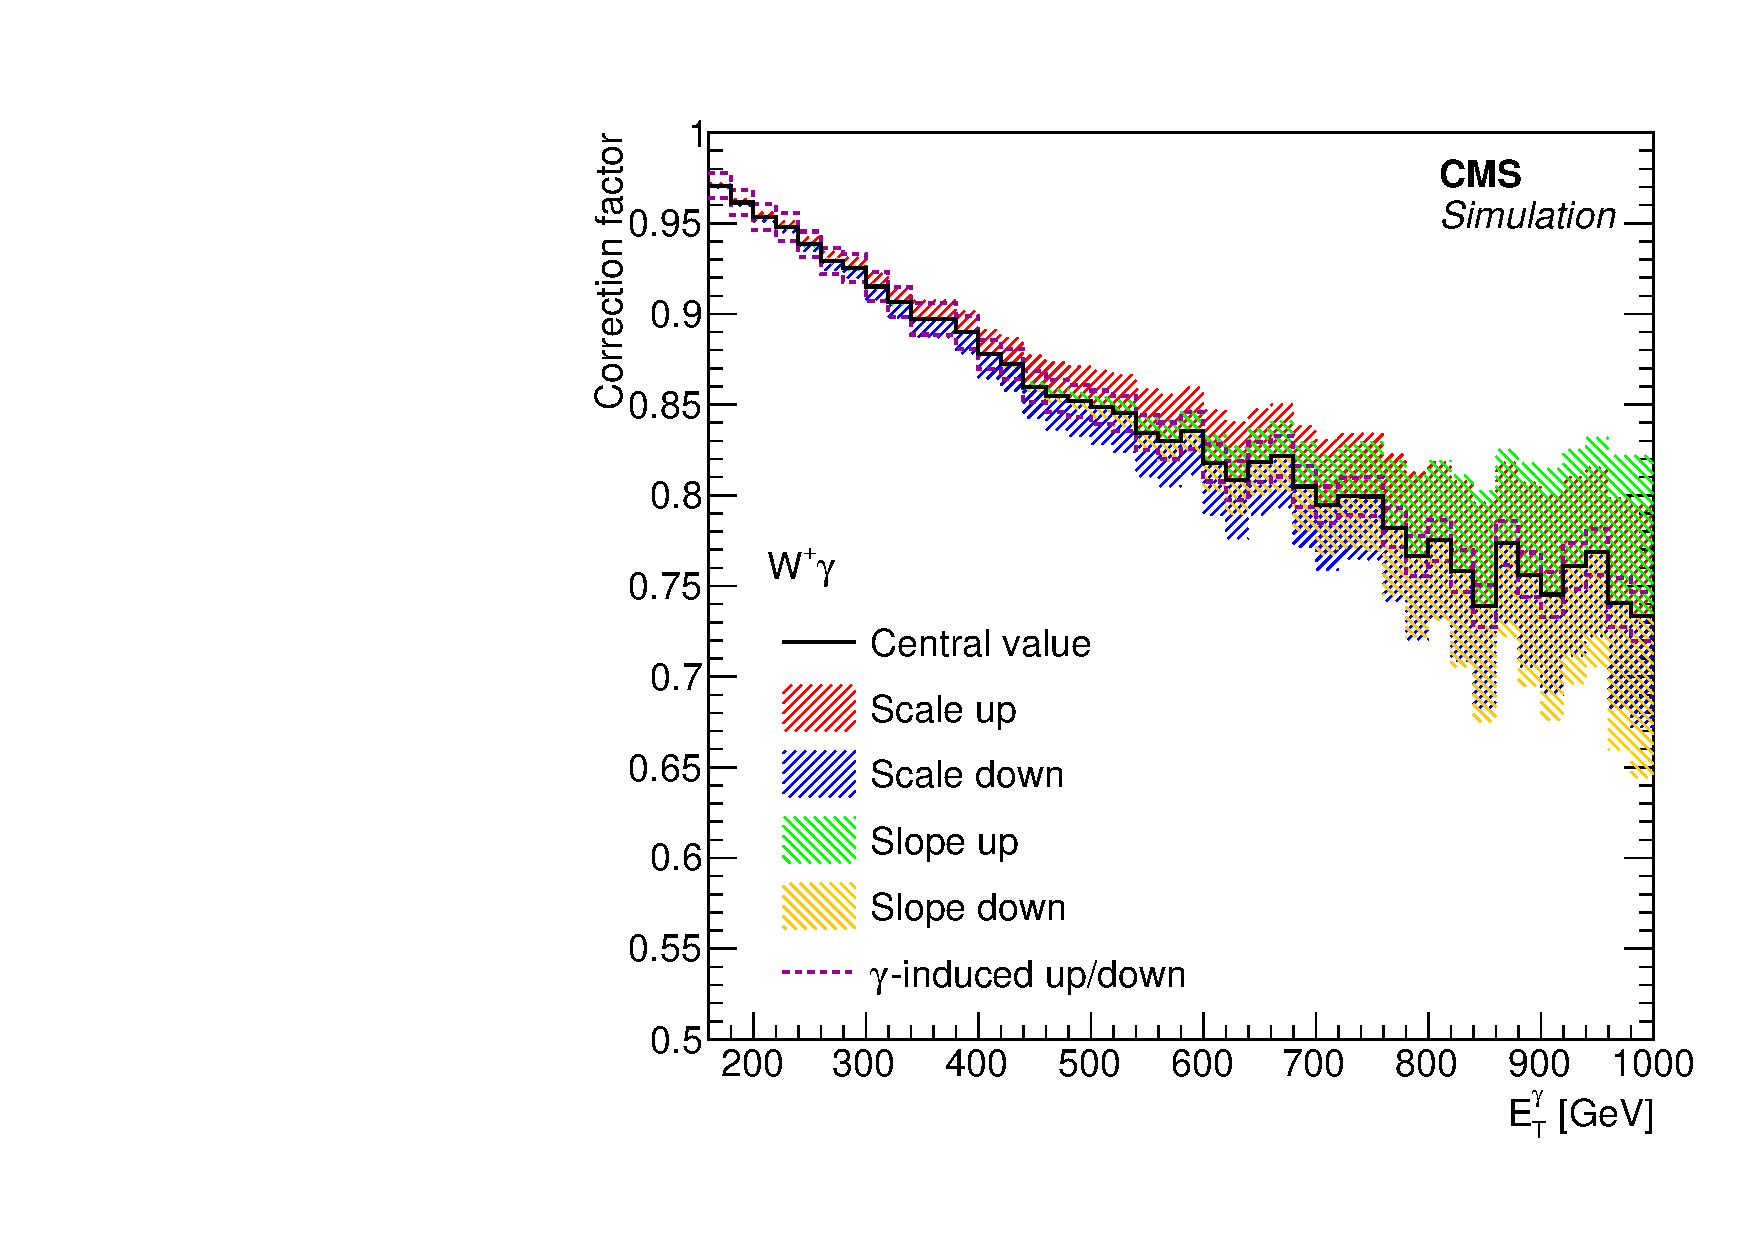
\includegraphics[width=0.32\textwidth]{Analysis/Figures/ewkcorr/wgplus.pdf}
  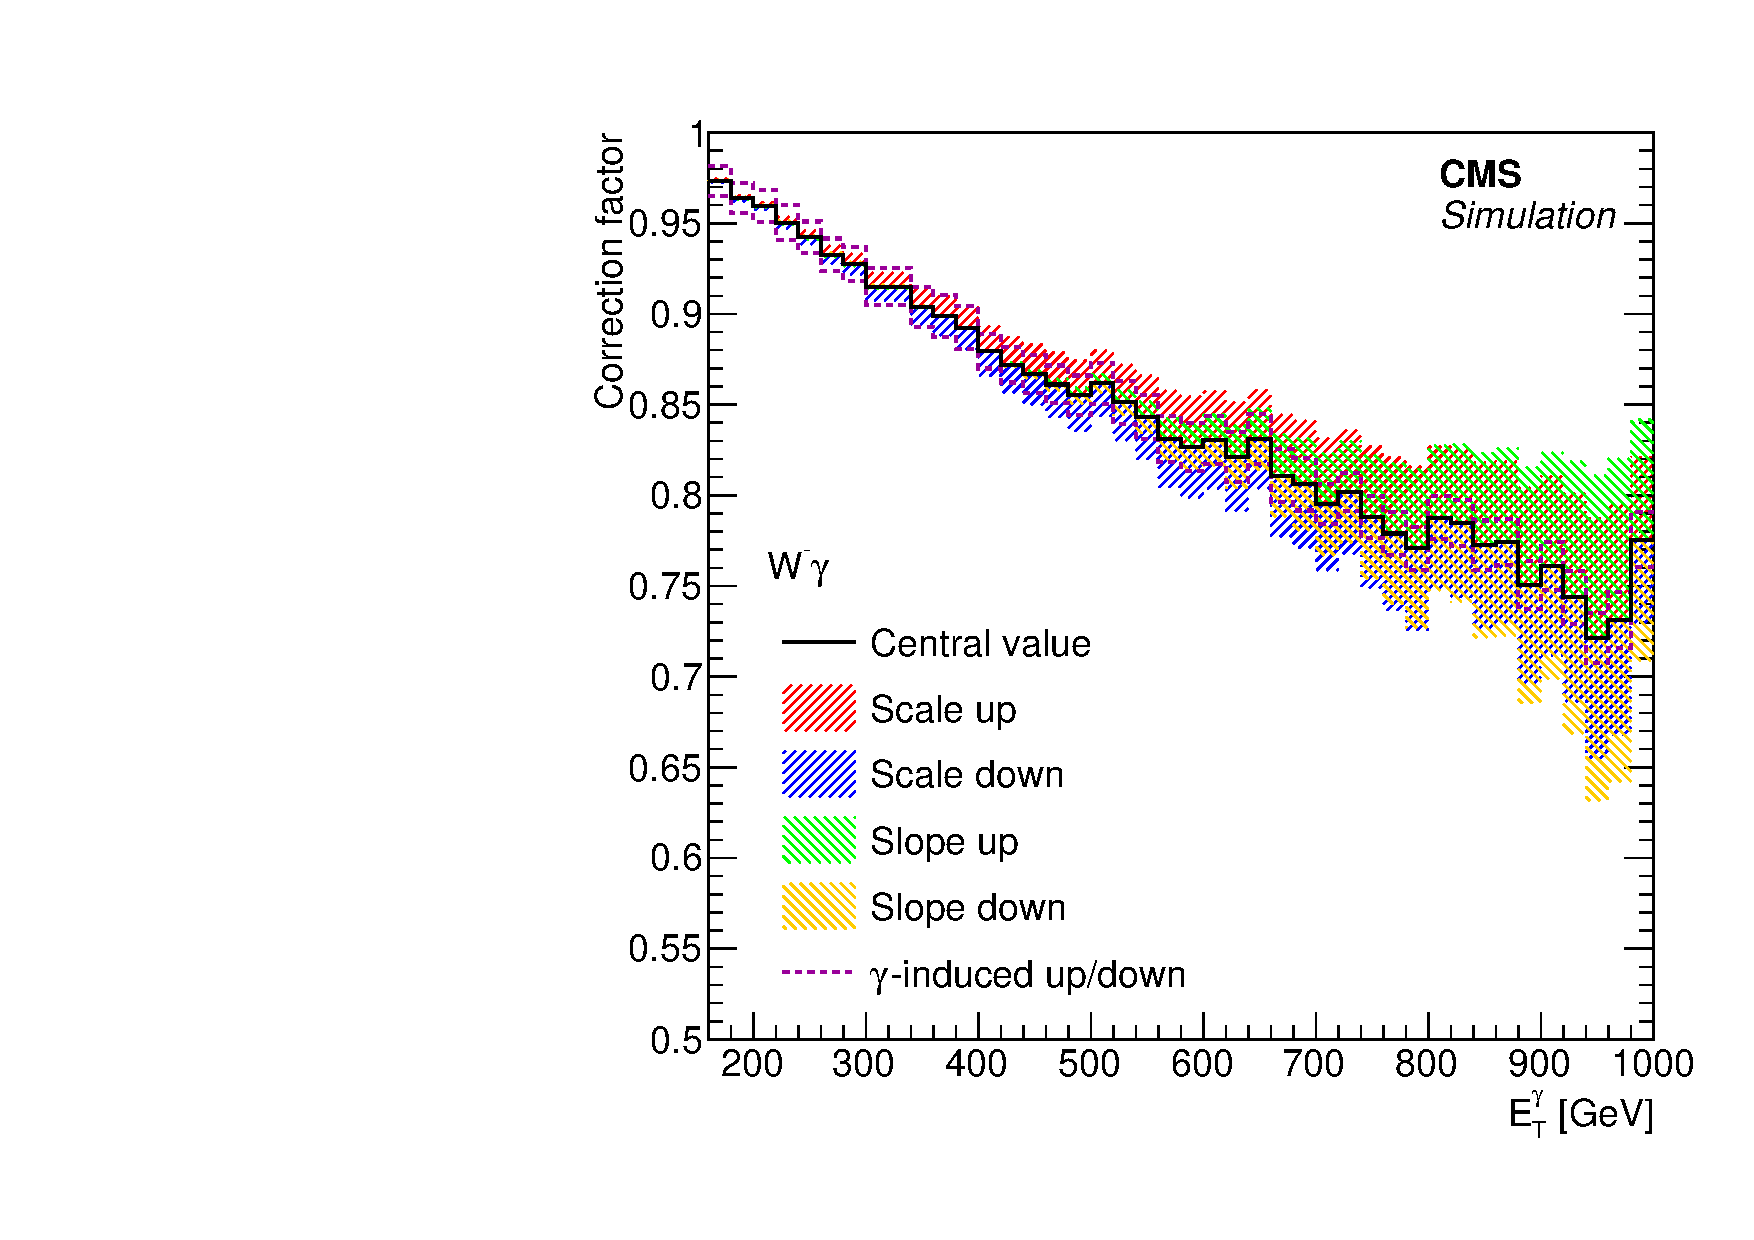
\includegraphics[width=0.32\textwidth]{Analysis/Figures/ewkcorr/wgminus.pdf}
  \caption{
    Electroweak NLO cross section corrections as a function of photon \pt\ for \zinvg\ (left), $\PW^{+}+\Pgg$ (middle), and $\PW^{-}+\Pgg$ (right) processes, overlaid with uncertainty bands. 
    See text for descriptions of the individual components of the uncertainty.
    The uncertainty due to \Pgg-induced production is negligible in \zinvg\ production.
  }
  \label{fig:ewk_correction}
\end{figure}

The differential cross section after the full higher-order corrections is
\begin{equation}
  % d\sigma^{\text{NNLO, NLO}}_{\text{QCD, EW}} =
  d\sigma^{\text{LO}}_{\text{QCD}} \cdot \kqcd \cdot \left(1 + \ksudakov + \kphoton \right),
\end{equation}
where $\kqcd = d\sigma^{\text{NNLO}}_{\text{QCD}} / d\sigma^{\text{LO}}_{\text{QCD}}$, and the two $k_{\text{EW}}$ terms are the Sudakov suppression and photon-induced enhancement components of the electroweak correction, respectively.

Furthermore, subtle differences between simulation and observation in the reconstruction and identification efficiencies for various particle candidates are accounted for with the set of selection efficiency correction factors $\rho$. 
The value of an individual $\rho$ typically lies within a few percent of unity. 
% Further details on the measurement and values of various $\rho$ are found in Chapter~\ref{chap:calibration}. %% gonna need to change

Four sources of systematic uncertainties considered for \ETg\ distribution ratios of the \vg\ processes are higher-order QCD corrections, higher-order EWK corrections, choice of PDF set, and data-to-simulation correction factors $\rho$. 
The four uncertainties are evaluated for each \ETg\ bin and fully correlated between the different bins.. 

The higher-order QCD renormalization and factorization scale uncertainties on the NNLO cross sections are assessed by varying the respective scales by factors 2 and 0.5 during the cross section computation. 
The uncertainties vary between 7-8\% across the bins and are considered uncorrelated in the ratio between the \zinvg\ and \wlng\ processes.

Theoretical uncertainties on the electroweak corrections are not well understood to date.  
We estimate the magnitude of the uncertainty on \ksudakov\ and \kphoton\ to be $\left(\ksudakov\right)^2$ and \kphoton, \ie, square of the correction for Sudakov suppression and the 100\% of the correction itself for the photon-induced enhancement. 
The choice of using the square of \ksudakov\ is motivated by the fact that fully resummed leading-log Sudakov suppression is an exponential of \ksudakov.
This prescription is motivated by discussions with J. Lindert based on the paper~\cite{}.

For the Sudakov suppression, which is the dominant term in the electroweak correction, we further consider two types of systematic variations, inspired by ref.~\cite{Lindert:2017olm}, which provides a prescription for electroweak correction uncertainties for $\mathrm{V}+\text{jets}$ processes. 
In this paper, electroweak correction as a function of the boson \pt\ is varied in overall scale and in slope. 
The slope variation is realized by selecting a point in the boson \pt\ spectrum and letting the shift in correction cross over at the point (see Figure~\ref{fig:ewk_correction_cartoon}). 
Following this prescription, we let the Sudakov suppression vary in overall scale and in slope, where we choose our crossover point for the slope variation to be at $\ETg=590\GeV$.

\begin{figure}[htbp]
  \centering
  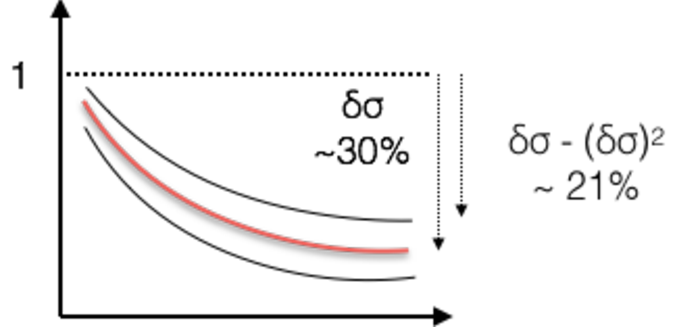
\includegraphics[height=0.3\textwidth]{Analysis/Figures/ewkcorr/scale.pdf}
  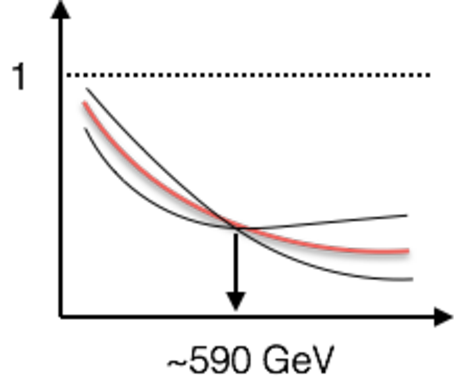
\includegraphics[height=0.3\textwidth]{Analysis/Figures/ewkcorr/shape.pdf}
  \caption{
    Electroweak correction variation scheme to cover the scale (left) and shape (right) uncertainties.
  }
  \label{fig:ewk_correction_cartoon}
\end{figure}

The PDF uncertainty is evaluated by varying the weight of each event using the weights provided in the NNPDF set, and taking the standard deviation of the resulting \ETg\ distributions. 
This uncertainty is considered fully correlated in the ratio between the \zinvg\ and \wlng\ processes, \ie, the variation of the ratio is bounded by the ratios formed by the simultaneous upward and downward variations of the numerator and denominator. .

Finally, data-to-simulation correction factors $\rho$ for the lepton identification efficiencies have associated uncertainties that do not cancel when taking ratios between regions defined by different lepton selection requirements.
The lepton efficiencies are measured using the ``tag-and-probe'' method where the tag object is an electron (muon) object passing the tight ID  and matched to a SingleElectron (SingleMuon) trigger and the probe object is a PF electron (muon) without any ID applied.
The passing (failing) categories are defined by events with probes passing (failing) the ID definition in question.
The electron (muon) scale factors $\rho$ are approximately unity with a flat 2\% (1\%) systematic uncertainty.

\subsection{Data-driven Control Regions}
\label{sec:control_regions}

Contributions from the \zinvg\ and \wlng\ processes are estimated using observed data in four mutually exclusive single-electron, single-muon, dielectron, and dimuon control regions.
The various ratios between the expected \zinvg\ yield in the combined signal regions and the expected \wlng\ and \zllg\ yields in the control region are constrained by MC simulations.
When a ratio is calculated using MC samples as a function of \ETg, it is referred to as the ``transfer factor'' between the two processes.
This background estimation method exploits the cancellation of some of the systematic uncertainties, both experimental and theoretical, in the transfer factors between the different  \vg\ processes.
 
For the transfer factor \RZll, the numerator is the expected \zinvg\ yield in the combined signal regions and the denominator is the expected \zllg\ yield in the relevant dilepton control region.
The uncertainties due to photon energy calibration, jet energy resolution, and higher-order QCD effects are significantly reduced on \RZll\ compared to when such effects are considered for individual processes. 
The only uncertainties in the transfer factor \RZll\ that do not largely cancel are those on lepton identification efficiency, the statistical uncertainty due to the limited MC sample size, and a minor uncertainty due to the different acceptances between the \zinvg\ and \zllg\ proccesses. 
Figure~\ref{fig:tf_z} shows the transfer factor \RZee\ (\RZmm) between the dielectron (dimuon) control region and the combined signal regions.

\begin{figure}[htbp]
  \centering
    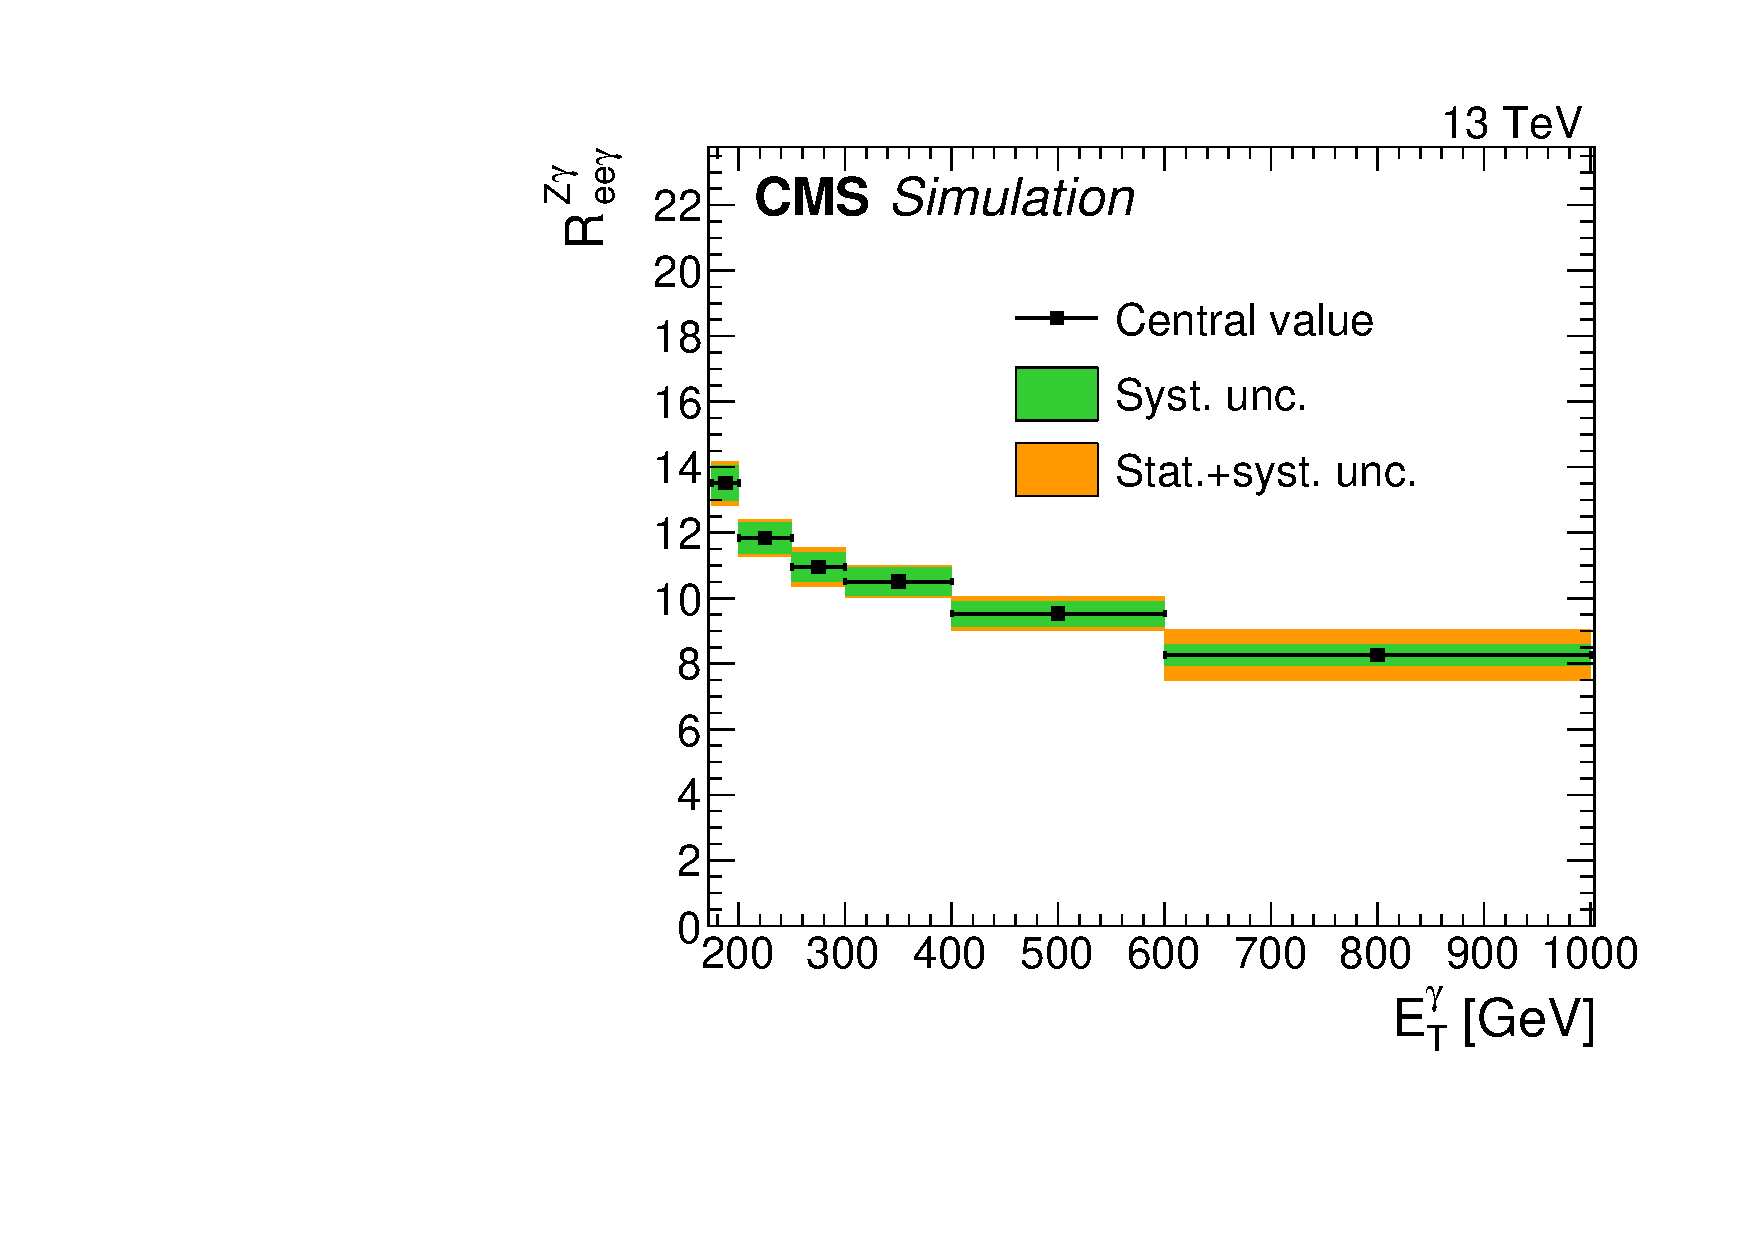
\includegraphics[width=0.49\textwidth]{Analysis/Figures/RZee.pdf}
    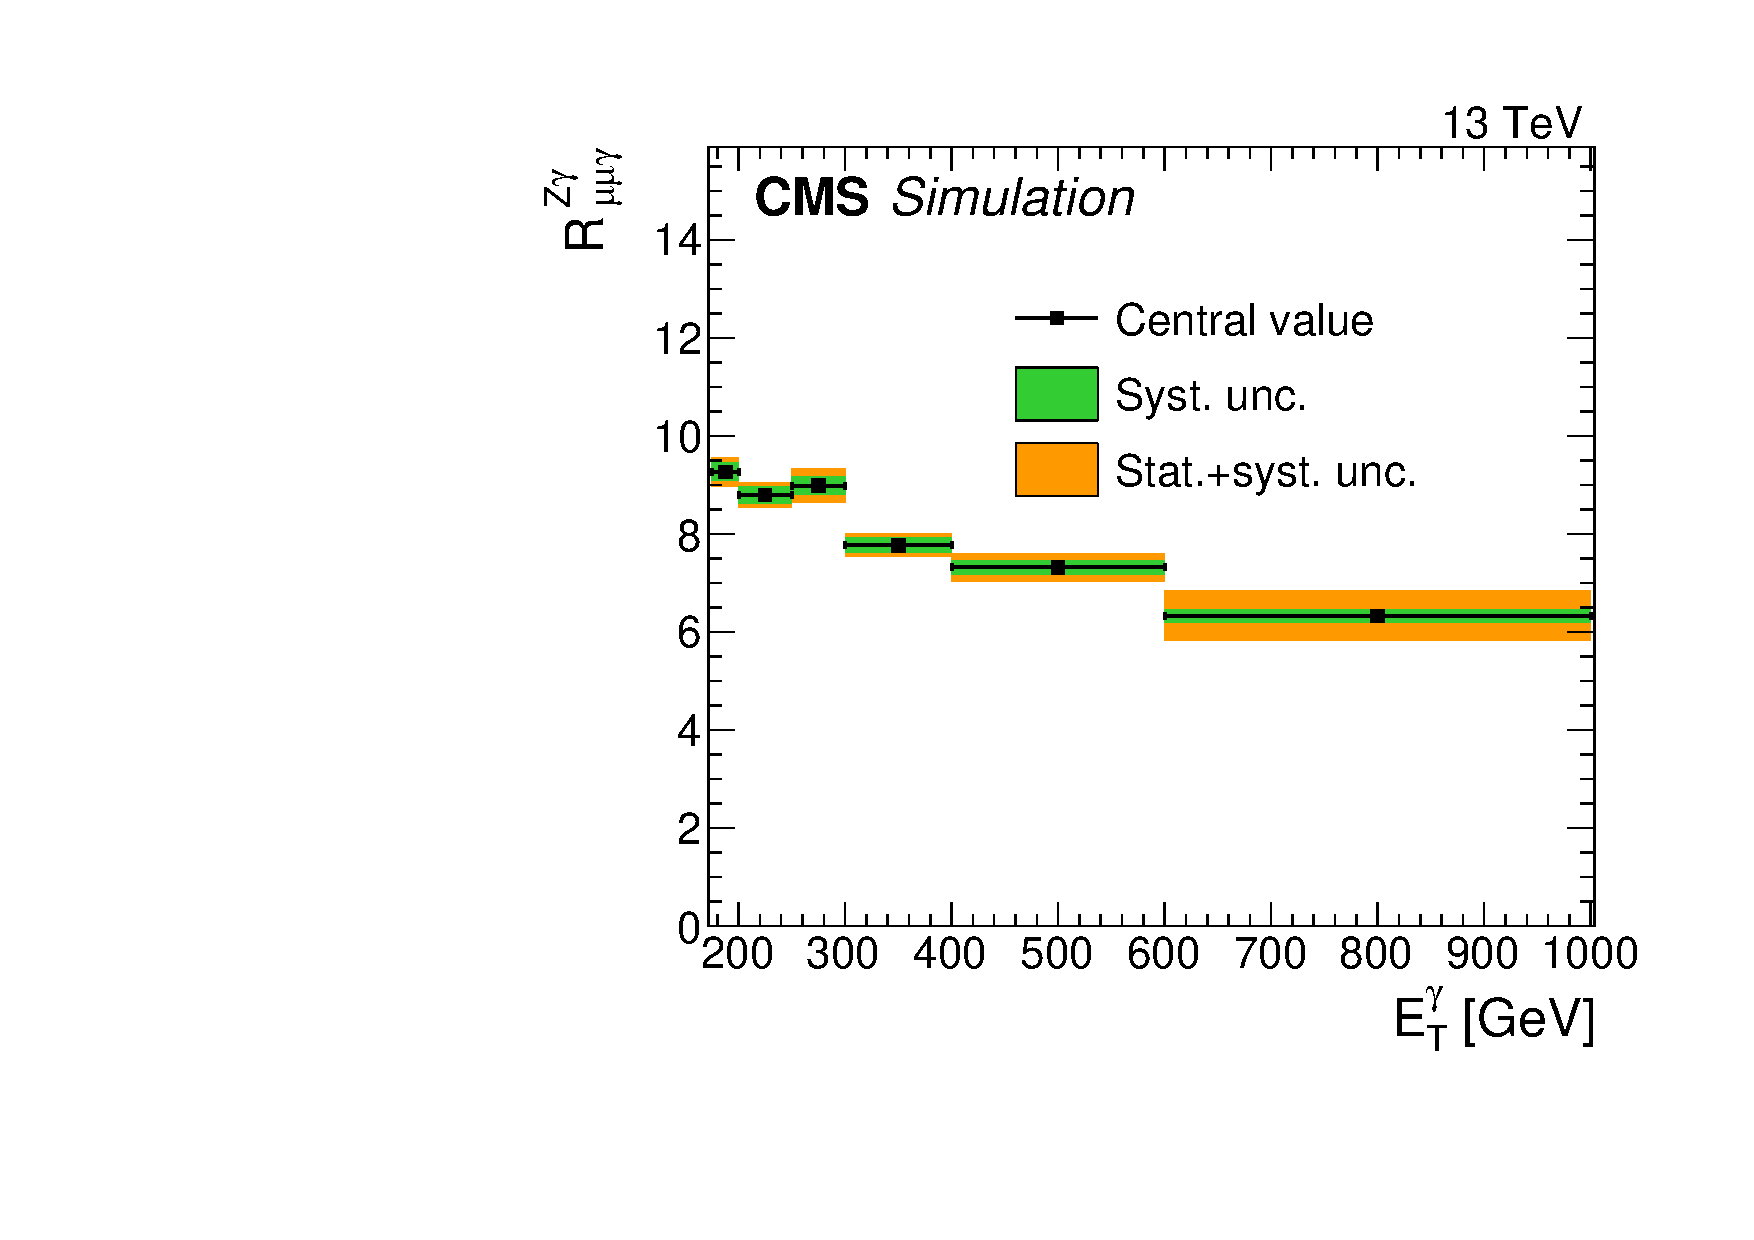
\includegraphics[width=0.49\textwidth]{Analysis/Figures/RZmm.pdf}
    \caption{
      Transfer factors \RZee\ (left) and \RZmm\ (right).
      The numerator is the expected \zinvg\ yield in the combined signal regions and the denominator is the expected \zllg\ yield in the dielectron (left) or dimuon (right) control region.
      The uncertainty bands in green (inner) and orange (outer) show the systematic uncertainty, and the combination of systematic and statistical uncertainty arising from limited MC sample size, respectively. 
      The systematic uncertainties considered are the uncertainties in the data-to-simulation correction factors $\rho$ for the lepton identification efficiencies.
    }
    \label{fig:tf_z}
\end{figure}

For increasing \ETg, the \PZ\ boson in a \zllg\ event tends to emerge with lower rapidity, and hence so do its decay products. 
As a consequence, the charged leptons are more likely to fall within the inner tracker acceptance, which increases the dilepton control region selection efficiency of these events. 
In contrast, the signal region selection efficiency of \zinvg\ events is unaffected by the rapidity of the final state neutrinos, as long as the observed \met\ has the appropriate magnitude and azimuthal direction. 
This causes the distinctive drop in the ratio \RZll\ with increasing \ETg.

Using the transfer factor \RZll, the total estimated event yield \Tll\ in each dilepton control region in the $i^\mathrm{th}$ bin of the \ETg\ distribution is given by
\begin{equation}
  \Tll[,i] = \frac{\NZg[i]}{\RZll[,i]} + b_{\ell\ell\Pgg,i},
\end{equation}
where \NZg\ is the predicted number of \zinvg\ events in the combined signal regions and $b_{\ell\ell\Pgg}$ is the predicted contribution from other background sources in the dilepton control region, namely \ttg, VV\Pgg, and misidentified hadrons. 
The subscript $i$ indicates that the quantities are evaluated in bin $i$ of the \ETg\ distribution.

Similar considerations apply to events arising from the \wlng\ process. 
A large fraction of such events are rejected by the electron and muon vetoes in the signal region selection and end up in the control regions instead. 
However, hadronic tau events and events where the leptons are out of acceptance or fail to be reconstructed will remain in the signal region, on top of the vetoes having imperfect efficiencies. 
In the ratio of these two classes of events, denoted \RWl, the only uncertainties that remain non-negligible are those associated with the lepton identification efficiency and the MC statistical uncertainty.

Table~\ref{tab:wg_breakdown} gives the breakdown of the \wlng\ background passing the full event selection for the signal region, categorized by the lepton flavor and, for the case of electrons and muons, the lepton pseudorapidity at the parton-level. 
From this breakdown, one sees that events where the \PW\ boson decays to a \Pgt\ and a neutrino constitute approximately 60\% of the \wlng\ background. 
The remaining 40\% of the \wlng\ background comes from events where the \PW\ boson decays to a \Pgm\ or \Pe\ and a neutrino.
Events containing an electron are more likely to be within the detector acceptance, while those with a muon are more likely to be out of acceptance.
For the in-acceptance background ($|\eta| < 2.5$), the identification efficiency, which is lower for electrons than for muons, which translates to a larger background contribution from the electrons. 
The requirement for large \met\ removes events with out-of-acceptance electrons because the energy from these electrons is captured by the calorimeters and retains events with out-of-acceptance muons because they contribute directly to the missing momentum.
The overall result is a larger background contribution from events with out-of-acceptance muons than from events with out-of-acceptance electrons. 
% Conversely, by requiring large \met, the muon $\eta$ distribution is highly skewed towards the edge of acceptance, driving the overall muon reconstruction efficiency in the sample lower and thereby making the background contributions from electrons and muons closer to each other. 

\begin{table}[tbp]
  \begin{center}
    \begin{tabular}{ l r | r r }
      \multicolumn{2}{ c |}{Subprocess} & \multicolumn{2}{| c }{$A\times\epsilon \times 10^{3}$} \\
      \hline
      \multicolumn{2}{ l |}{$\PW\rightarrow\Pe\Pgn + \Pgg$} & 1.68 & \\
      & $|\eta^{\Pe}| < 2.5$ & & 1.35 \\
      & $|\eta^{\Pe}| > 2.5$ & & 0.32 \\
      \hline
      \multicolumn{2}{ l |}{$\PW\rightarrow\Pgm\Pgn + \Pgg$} & 1.83 & \\
      & $|\eta^{\Pgm} < 2.5$ & & 0.74 \\
      & $|\eta^{\Pgm} > 2.5$ & & 1.08 \\
      \hline
      \multicolumn{2}{ l |}{$\PW\rightarrow\Pgt\Pgn + \Pgg$} & 5.03 & \\
    \end{tabular}
    \caption{
      The breakdown of simulated $\PW+\Pgg$ events passing the full event selection. 
      Events are categorized in the \PW\ decay mode. 
      Events with \Pe\Pgn\ and \Pgm\Pgn\ final states are further divided into those where the lepton is roughly within acceptance ($|\eta| < 2.5$) but failed the lepton veto, and those where the lepton is out of acceptance ($|\eta| > 2.5$). 
      For each \PW\ decay mode, the fraction out of total generated ($A\times\epsilon$) is shown.
    }
    \label{tab:wg_breakdown}
  \end{center}
\end{table}

Figure~\ref{fig:tf_w} shows the transfer factor \RWe\ (\RWm) between the single-electron (single-muon) control region and the combined signal regions, for which the numerator is the estimated \wlng\ yield in the combined signal regions, and the denominator is the estimated \wlng\ yield in the relevant control region. 
The ratio \RWl\ decreases with increasing \ETg\ in a similar manner to \RZll.
The underlying logic is the same; e.g., that the signal region selection efficiency is unaffected by \ETg\ while the control region acceptances increase with increasing \ETg\ due to increased lepton efficiency resulting from lower \PW\ rapidity. 

\begin{figure}[htbp]
  \centering
    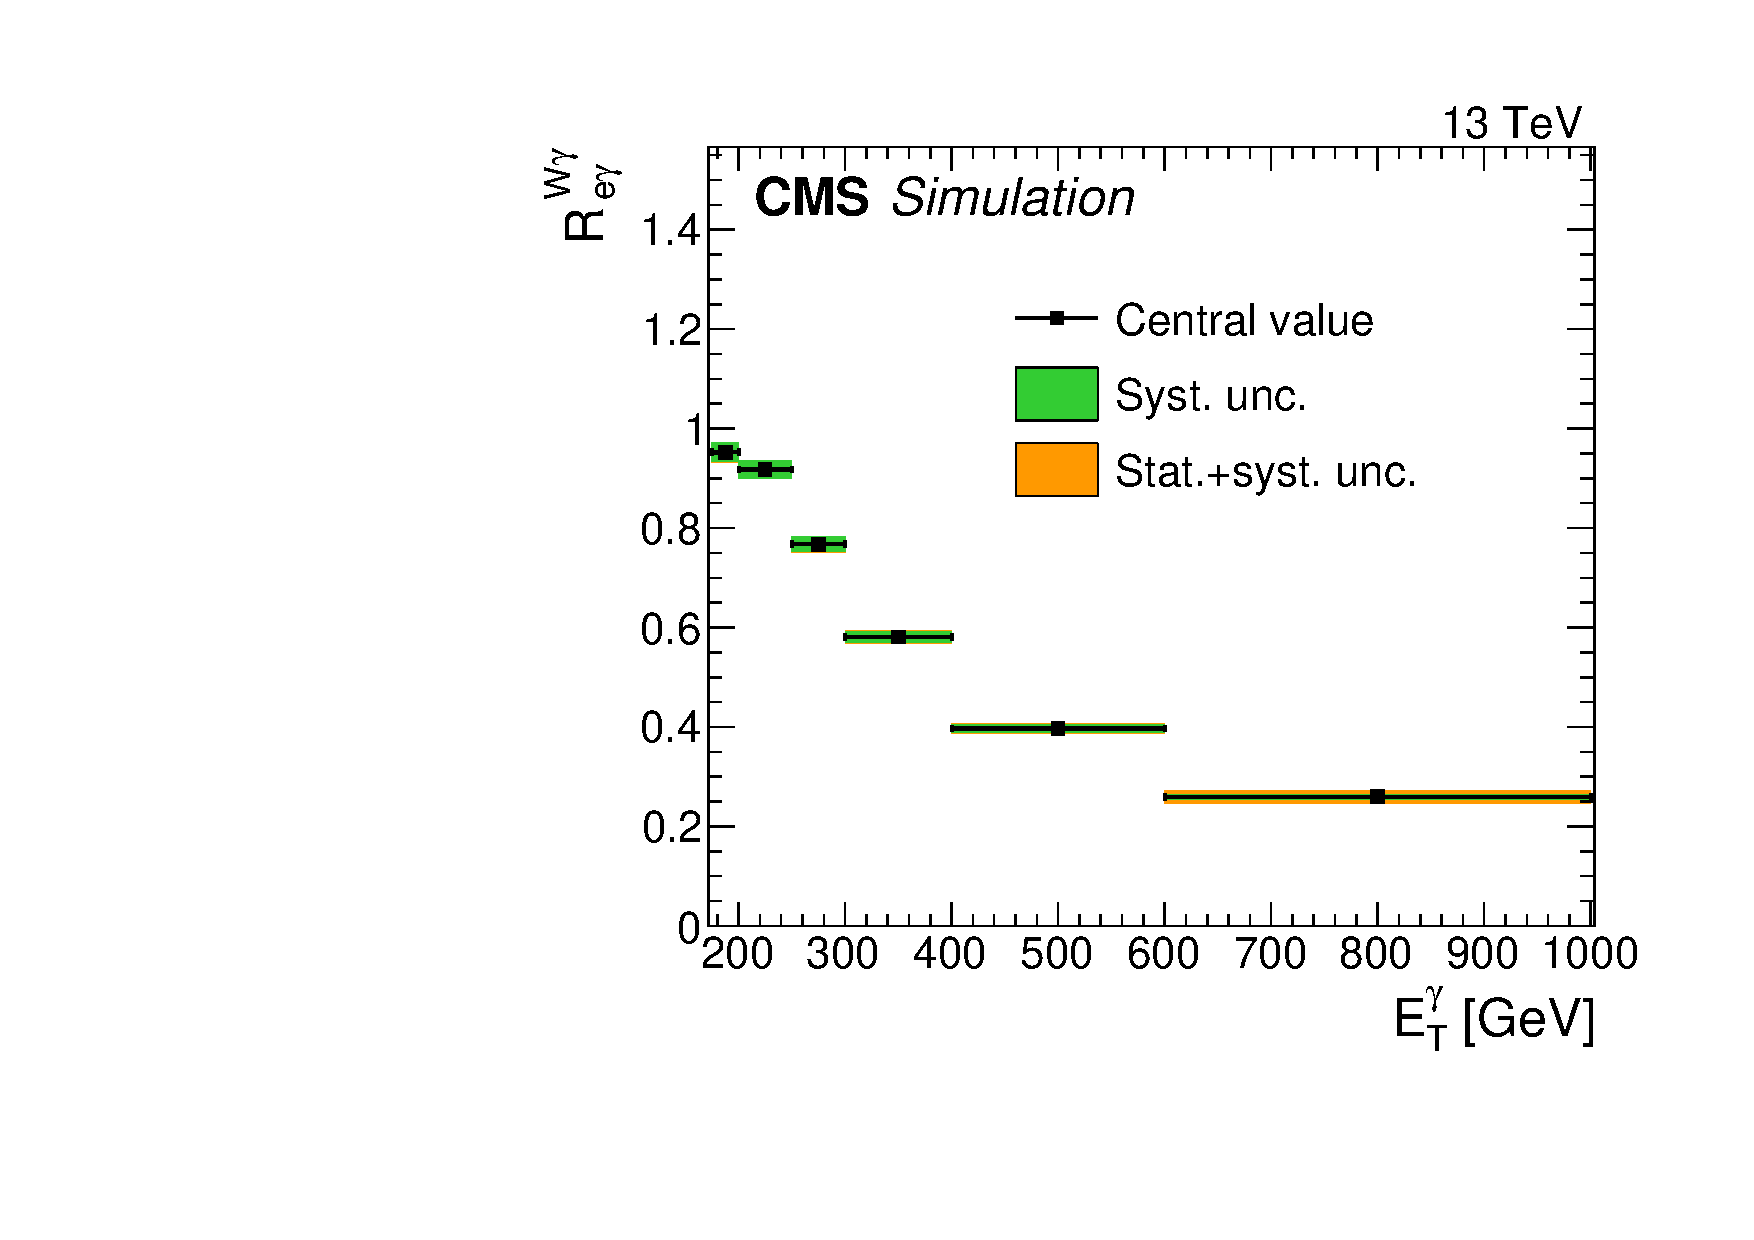
\includegraphics[width=0.49\textwidth]{Analysis/Figures/RWe.pdf}
    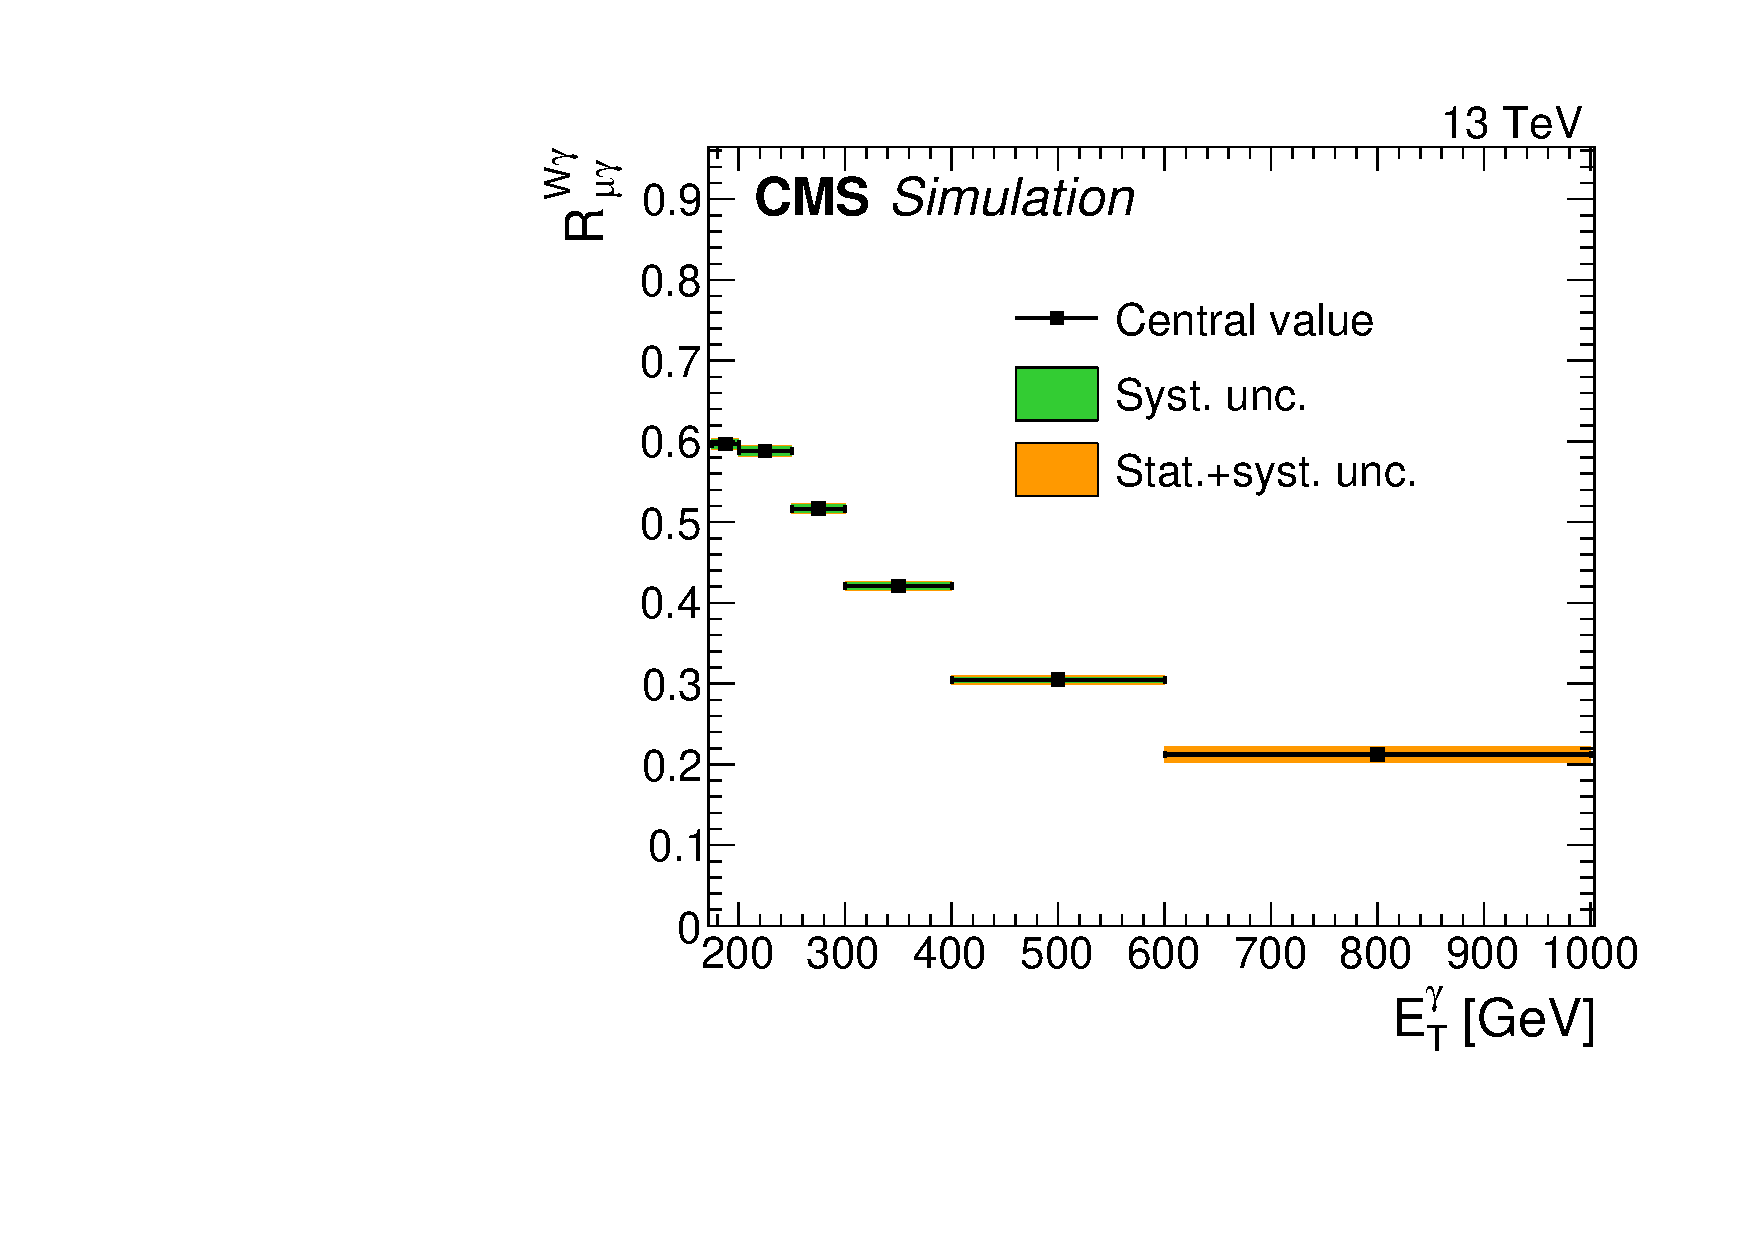
\includegraphics[width=0.49\textwidth]{Analysis/Figures/RWm.pdf}
    \caption{
      Transfer factors \RWe\ (left) and \RWm\ (right).
      The numerator is the expected \zinvg\ yield in the combined signal regions and the denominator is the expected \wlng\ yield in the mono-electron (left) or mono-muon (right) control region.
      The uncertainty bands in green (inner) and orange (outer) show the systematic uncertainty, and the combination of systematic and statistical uncertainty arising from limited MC sample size, respectively. 
      The systematic uncertainties considered are the uncertainties in the data-to-simulation correction factors $\rho$ for the lepton identification efficiencies.
    }
    \label{fig:tf_w}
\end{figure}

Finally, to benefit further from the larger statistical power that the single-lepton control samples provides, an additional transfer factor $\fZW = \NZg / \NWg$ is defined to connect the \zinvg\ and \wlng\ background yields in the signal regions, where the quantity $\NWg$ is the number of \wlng\ events in the combined signal regions. 
When calculating the ratio \fZW, all experimental uncertainties associated with the data-to-simulation correction factors $\rho$ cancel since both processes result in very similar event configurations. 
The main uncertainties in \fZW\ are those from higher-order theoretical corrections, discussed in Section~\ref{sec:vgmc}.
Figure~\ref{fig:tf_syst} shows the effect of each systematic uncertainty in \fZW\ with respects to its nominal value for \zinvg\ and \wlng, respectively.

\begin{figure}[htbp]
  \centering
    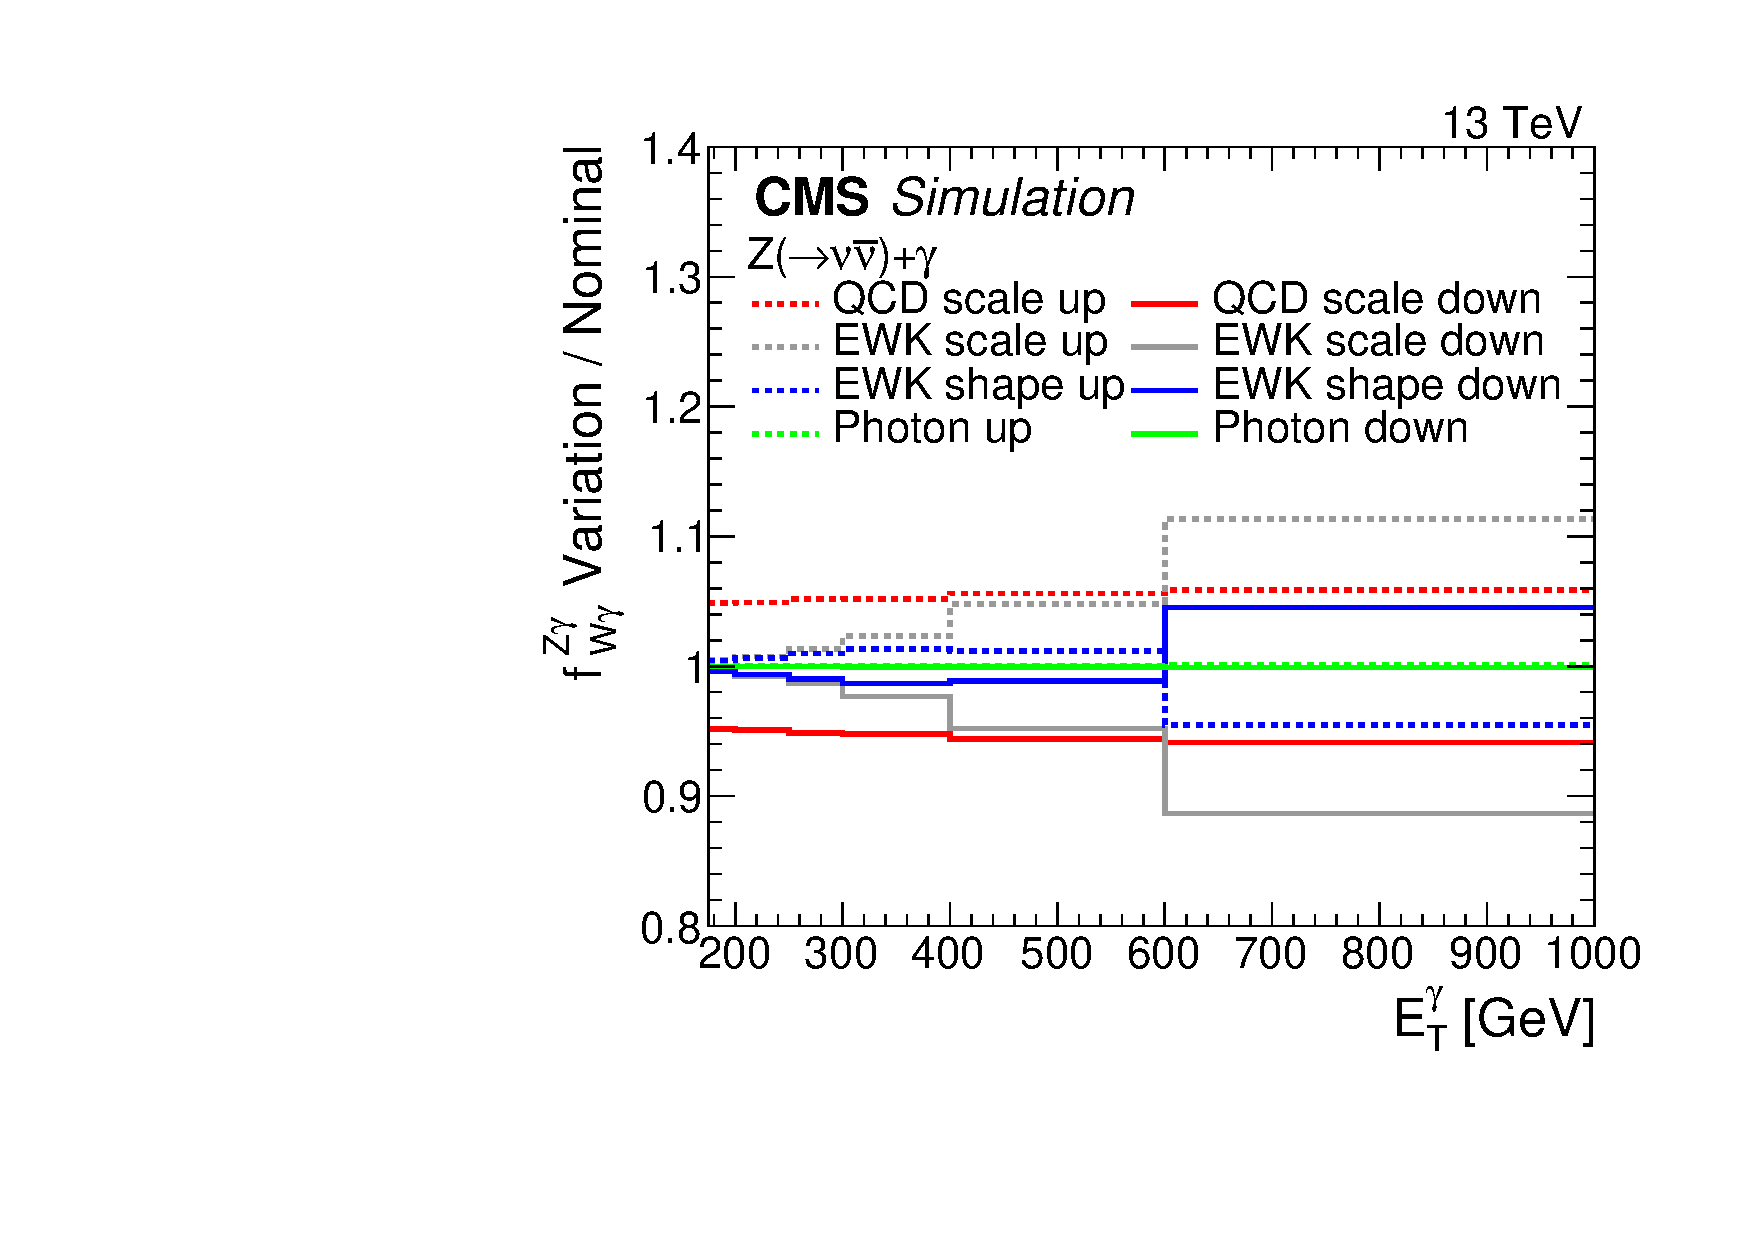
\includegraphics[width=0.49\textwidth]{Analysis/Figures/tf_syst_zg.pdf}
    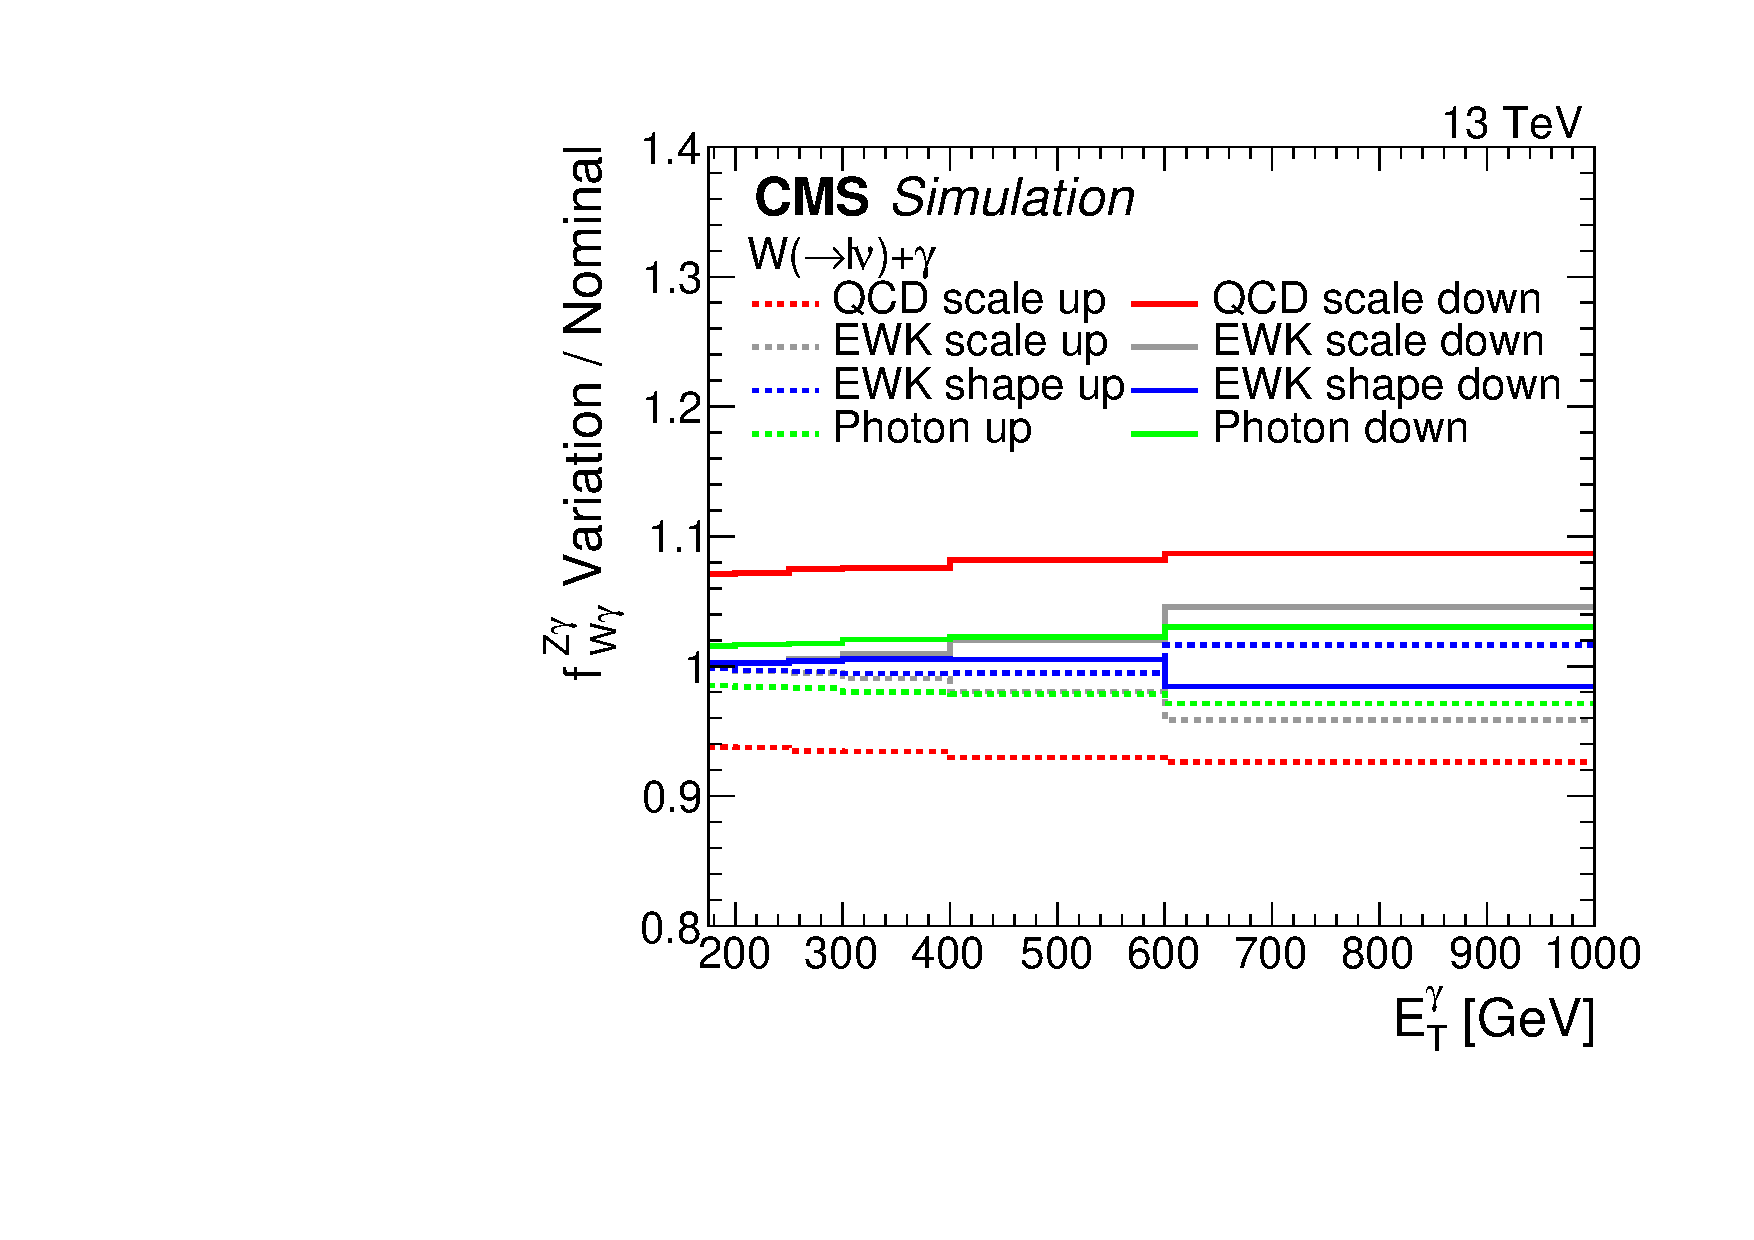
\includegraphics[width=0.49\textwidth]{Analysis/Figures/tf_syst_wg.pdf}
    \caption{
      Systematic uncertainty in the transfer factors for \zinvg\ (left) and \wlng\ (right). The last bin includes all events with $\ETg > 1000\GeV$.
    }
    \label{fig:tf_syst}
\end{figure}

The ratio \fZW\ rises rather than falls with increasing \ETg\ because \wlng\ events have a lower signal region selection efficiency when the charged lepton falls within the tracker acceptance due to the lepton veto while the \zinvg\ efficiency is independent of \ETg.
Figure~\ref{fig:tf_wz} shows the transfer factor \fZW\ between the \zinvg\ and \wlng\ processes in the combined signal region.


\begin{figure}[htbp]
  \centering
    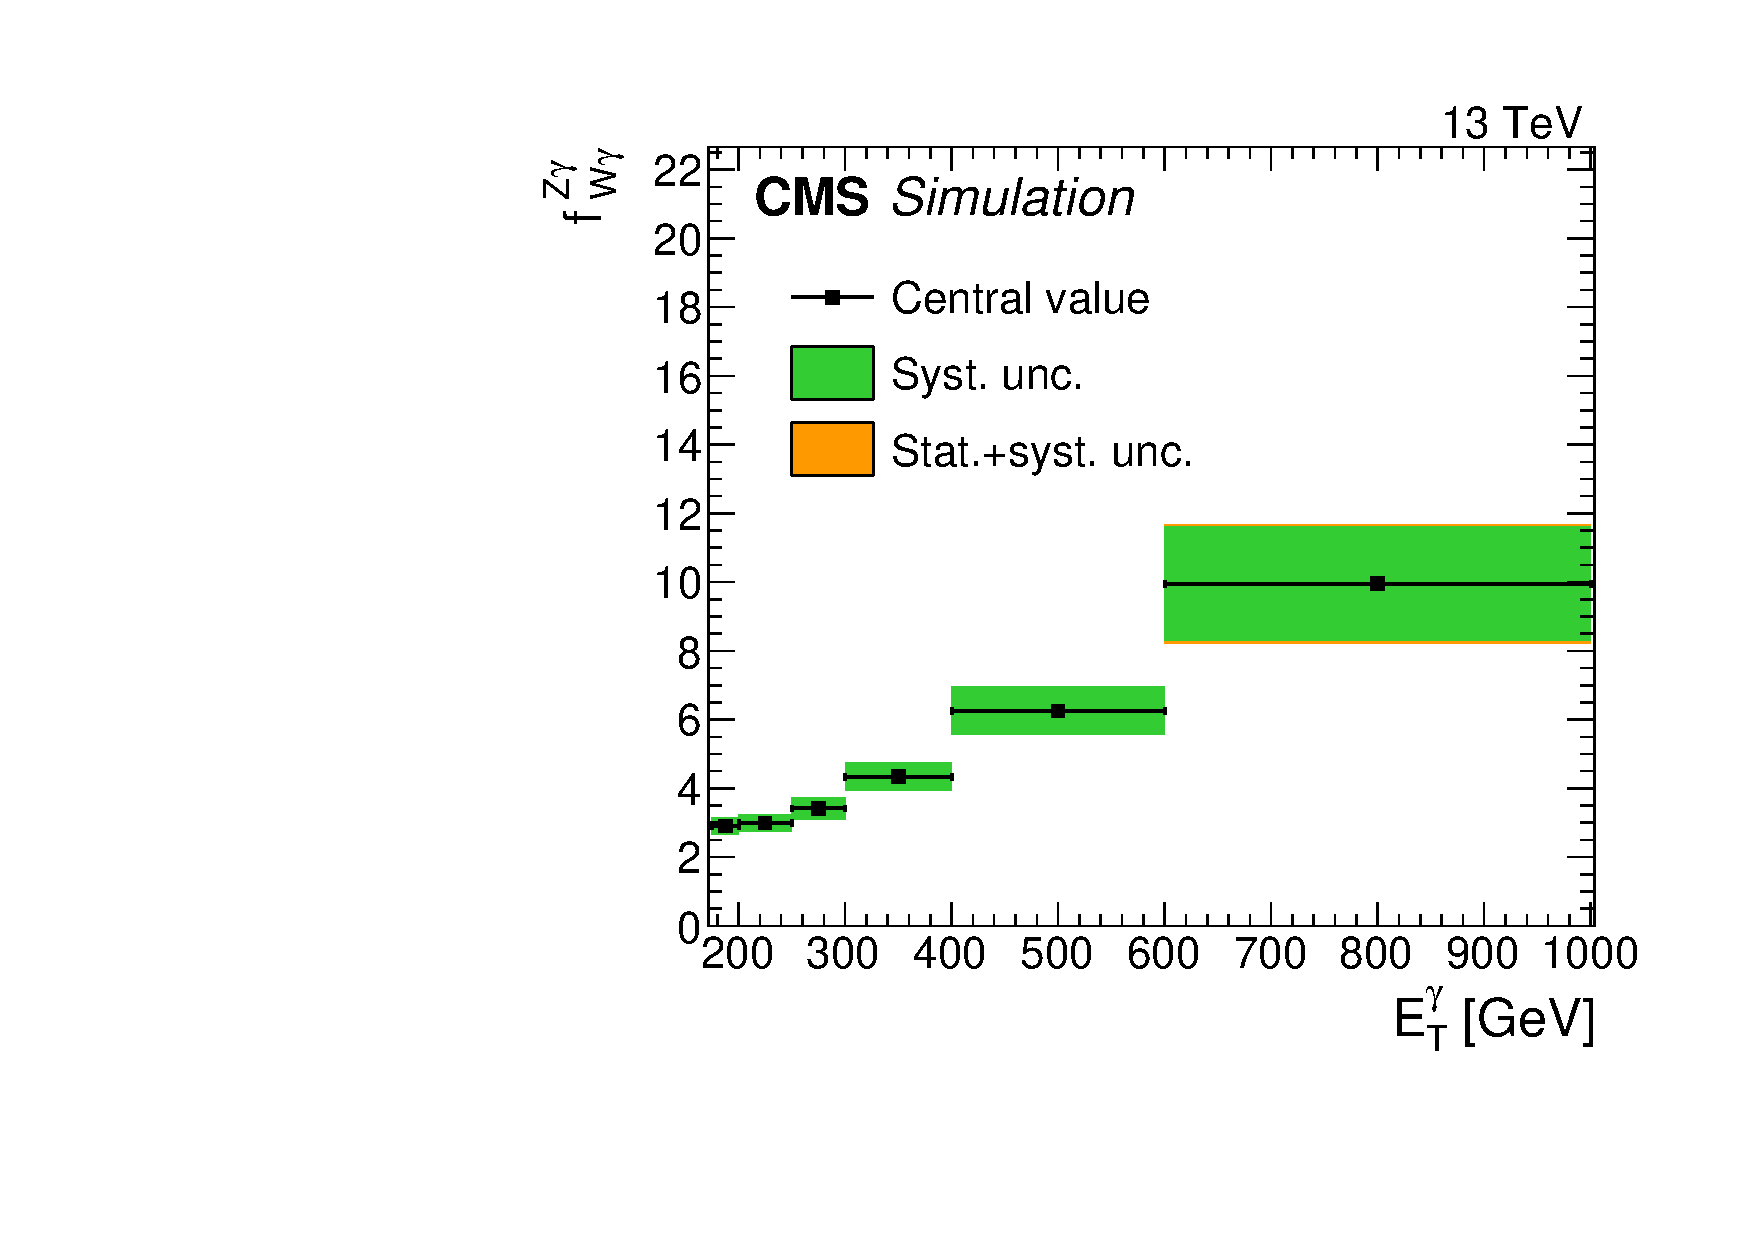
\includegraphics[width=0.49\textwidth]{Analysis/Figures/fZW.pdf}
    \caption{
      Transfer factor \fZW in the combined signal regions.
      The numerator is the expected \zinvg\ yield and the denominator is the expected \wlng\ yield.
      The uncertainty bands in green (inner) and orange (outer) show the systematic uncertainty, and the combination of systematic and statistical uncertainty arising from limited MC sample size, respectively. 
      The systematic uncertainties considered are the uncertainties from higher-order theoretical corrections.
    }
    \label{fig:tf_wz}
\end{figure}

Using \RWl\ and \fZW, the total estimated event yield \Tl\ in each single-lepton control region in the $i^\mathrm{th}$ bin of the \ETg\ distribution is given by
\begin{equation}
  \Tl[,i] = \frac{\NZg[i]}{\RWl[,i]\fZW[,i]} + b_{\ell\Pgg,i},
\end{equation}
where $b_{\ell\Pgg}$ is the predicted contribution from other background sources in the single-lepton regions, namely misidentified electrons and hadrons and other minor SM processes.
